% Compile with XeLaTeX (Overleaf) or Tectonic (locally); see README.md in this directory.
% DSA5208 Project 2 report source.
\documentclass[lang=en,11pt,a4paper,bibend=bibtex]{elegantpaper}
\usepackage[english]{babel}
\usepackage{tabularx}
\usepackage{array}
\usepackage{float}
\usepackage{needspace}
\usepackage{microtype}
\usepackage{xurl}
\usepackage{multirow}
\geometry{left=25mm,right=25mm,top=22mm,bottom=24mm}
\linespread{1.16}
\setlength{\parskip}{3pt}
\setlength{\parindent}{1.5em}
\setlength{\emergencystretch}{2em}
\widowpenalty=10000
\clubpenalty=10000
\raggedbottom
\captionsetup{font=small,labelfont=bf,justification=raggedright,singlelinecheck=false}
\newcolumntype{Y}{>{\raggedright\arraybackslash}X}
\lstset{language=bash,basicstyle=\small\ttfamily,keywordstyle=\color{black},
  frame=none,backgroundcolor=\color{lightgrey},breaklines=true,
  columns=fullflexible,keepspaces=true,showstringspaces=false,
  xleftmargin=8pt,xrightmargin=8pt,aboveskip=10pt,belowskip=10pt}
\graphicspath{{../../reports/figures/}{figures/}}
\newcommand{\memberA}{Jia Siqi (A0333724H)}
\newcommand{\memberB}{Jia Zeyue}
\newcommand{\mm}{\,mm}
% Final model on the original (not QC'd) 2024 rows, from reports/final_model_on_original_2024.json.
\newcommand{\FinalOrigROC}{.940}
\newcommand{\FinalOrigPR}{.648}
\newcommand{\FinalOrigBSS}{.450}
\newcommand{\FinalOrigFone}{.616}
\newcommand{\AIUsage}{The research ideas, the modelling approach, the evaluation design (temporal split, validation-based selection and metrics) and all key decisions are our own. We cleaned the data, built the feature pipeline and the baseline models, and reviewed every result. Anthropic's Claude Code assisted under our direction: it implemented the quality-control rules, the threshold-free and amount models and the scripts that evaluate them, and the Task~1 analysis; it also ran the Spark experiments, produced the figures, and helped draft and typeset this report. Every number in this report comes from the scripts and saved reports in the repository.}
\hypersetup{pdftitle={Singapore Rainfall 2017--2024: Patterns and 30-Minute Exceedance Forecasts},
  pdfauthor={Jia Siqi and Jia Zeyue}}
\title{Singapore Rainfall 2017--2024:\\Patterns and 30-Minute Exceedance Forecasts}
\author{\memberA\qquad \memberB}
\institute{DSA5208 Project 2, National University of Singapore}
\date{18 October 2026}
\begin{document}
\maketitle
\vspace{0.3em}

\section{Overview}
We analyse the five-minute rain-gauge records of the National Environment Agency for 2017--2024 \hyperref[ref:1]{[1]} with Apache Spark. \textbf{Task~1} describes how rainfall changes within a year, across the island and between years. \textbf{Task~2} builds one Spark MLlib model that returns, for any station $s$, prediction time $t$ and threshold $r$,
\[
P\big(Y_{s,t} > r\big),\qquad Y_{s,t} = \text{rainfall at } s \text{ in } (t,\,t+30\text{ min}].
\]
The final model multiplies a gradient-boosted probability of any rain by a neural-network distribution of the amount. On the 2024 test year it has a Brier skill score of 0.45 at $r=1$\mm{} and 0.12 at 20\mm{} against climatology, and its probabilities are calibrated from 0.2 to 20\mm{} (Section~\ref{sec:results}). Sections~\ref{sec:data}--\ref{sec:task1} cover the data, computing environment, cleaning and Task~1; Sections~\ref{sec:features}--\ref{sec:results} cover feature selection, model development and results; Section~\ref{sec:limits} discusses validity checks and limitations.

\section{Data, computing environment and cleaning}\label{sec:data}
\subsection{Data}
The eight annual files contain \textbf{48,538,713 readings} from 91 stations; between 54 and 80 stations report in any one year. Each reading is the rain collected in the five minutes ending at its timestamp (Singapore time, SGT). Tipping-bucket gauges report multiples of about 0.2\mm{}; 323,342 readings lie off the 0.2\mm{} lattice because 24 gauges have calibrated tips of 0.197--0.204\mm. These are kept. 97\% of readings are zero.

\subsection{Computing environment}
All Spark jobs for Task~1, the threshold-free models and the final model ran on one laptop in Spark local mode (Table~\ref{tab:env}). The data fit on one machine after conversion to Parquet, and local mode uses the same DataFrame and MLlib code as a cluster: only the \texttt{--master} argument would change. The single-threshold baselines of Section~\ref{sec:baselines} were trained by a group member on a Linux workstation with \texttt{local[4]} and a 6\,GB driver. Because the laptop was shared between jobs, every full-scale job took a file lock (\texttt{lockf}), so at most one Spark application ran at a time.

\begin{table}[H]
\centering\small
\caption{Computing environment and run times of the main stages.}\label{tab:env}
\renewcommand{\arraystretch}{1.15}
\begin{tabularx}{\linewidth}{@{}p{0.24\linewidth}Y@{}}
\toprule
Hardware & MacBook Air (Apple M5, 10 cores: 4 performance + 6 efficiency), 24\,GB RAM, macOS 26.5 \\
Spark & Apache Spark 4.0.1 (PySpark), \texttt{local[10]}, driver heap 7--9\,GB, 40 shuffle partitions, adaptive query execution, session time zone Asia/Singapore \\
Software & OpenJDK 17.0.20; Python 3.12.13; NumPy 2.5.3, pandas 3.0.6, PyArrow 25.0.1 (Spark pandas UDFs), SciPy 1.18.1, Matplotlib 3.11.2 \\
Storage & raw CSV 7.5\,GB; cleaned Parquet 3.3\,GB; feature tables 2.6\,GB (2.4\,GB more after QC) \\
\midrule
Run times & quality control of all years 3.5\,min; fitting the ZILN model (three GBTs, 33.7\,M training rows) 28\,min; fitting the MLP amount model (2.04\,M wet rows) 33\,min; Task~1 aggregation about 15\,min; one prediction, including Spark start-up, 13\,s \\
\bottomrule
\end{tabularx}
\end{table}

\subsection{Cleaning}
\texttt{clean\_rainfall.py} reads each CSV with an explicit schema and writes partitioned Parquet. A record would be rejected for an unparseable timestamp, missing station, negative or non-numeric rainfall, invalid coordinates or an unexpected unit, and duplicate (station, timestamp) records are resolved by the newest update time. No reading failed these checks and no exact duplicates exist. Three properties of the source needed care:
\begin{itemize}[leftmargin=1.5em,itemsep=3pt]
\item \textbf{Timestamps.} 1,775,327 readings (3.7\%, nearly all in 2017) are stamped one second before the five-minute mark (\texttt{hh:mm:59}). Every reading is assigned to its nominal five-minute slot; afterwards 86 slots hold two readings, all with equal values.
\item \textbf{Gaps.} 3.75\,M station-slots (7.2\% of those expected) are missing, 29\% of them in 2018 (Fig.~\ref{fig:coverage}). Gaps are never filled with zeros. A prediction row is used for training or evaluation only if the station's previous 60 minutes and the 30-minute target window are completely observed; 46.99\,M rows qualify. The reading after a gap of an hour or more is wet less often than other readings (2.0\% vs 2.9\%) and is not unusually large, so a gap is rain lost rather than rain reported late. Task~1 therefore works with rates per observed reading.
\item \textbf{Target precision.} The target is the sum of six readings. Summing doubles gives values such as $5\times0.4 = 2.0000000000000004$, and the 2024 file stores some readings of 8--10\mm{} with float32 noise (8.60001). Either error turns a total of exactly $r$ into ``$>r$''. This affected about 3,500 labels a year at thresholds of 1.4\mm{} and above. We round the target to 0.001\mm, the resolution of the readings, and refitted the final amount model on the corrected labels. A recomputation from slot-exact readings matches the target on all 47.0\,M rows.
\end{itemize}

\subsection{Quality control}\label{sec:qc}
The portal warns that the data have not been quality controlled \hyperref[ref:1]{[1]}, and inspection of the training years found faulty gauges: stations reading zero for weeks while their neighbours had heavy rain (S24B in Jan--Apr 2017, S84 in Dec 2019, S226 in Mar 2021) and isolated extremes (S107 reported 438 and 482\mm{} on 20--21 Aug 2022 while its neighbours recorded little rain). \texttt{qc.py} masks such readings with the fixed rules in Table~\ref{tab:qc}. They use only rainfall readings, never model output, and apply identically to every year. Each station is compared with up to eight neighbours within 10\,km; a neighbour's daily total counts only the hours in which the station itself reported.

\begin{table}[H]
\centering\small
\caption{Quality-control rules. The thresholds were fixed to catch the faults listed above without flagging ordinary heavy convective days, before any model was trained on the QC'd data.}\label{tab:qc}
\renewcommand{\arraystretch}{1.15}
\begin{tabularx}{\linewidth}{@{}p{0.17\linewidth}Yp{0.17\linewidth}@{}}
\toprule
\textbf{Rule} & \textbf{Flags} & \textbf{Masked} \\
\midrule
A stuck zero & a run of exact-zero station-days with $\ge 3$ days on which the neighbour median was $\ge 5$\mm & whole run \\
B isolated extreme & station-day $\ge 100$\mm{} while the wettest neighbour got $<15\%$ of it & day $\pm 1$ \\
C phantom rain & station-day $\ge 20$\mm{} with $\ge 1$\mm{} in $\ge 3$ hours while the wettest of $\ge 5$ neighbours got $\le 5\%$ of it & day $\pm 1$ \\
D repeat & $\ge 3$ B/C days at one station, $\le 30$ days apart & whole span $\pm 1$ day \\
E spike & one 5-min value $\ge 5$\mm, both adjacent readings $<10\%$ of it, no neighbour reading $\ge 1$\mm{} within $\pm 30$\,min & that slot \\
\bottomrule
\end{tabularx}
\end{table}
The rules raise 110 flags and remove 313,976 readings (0.65\%). The largest fault was not on the manual list: S36 read zero from December 2018 to August 2020 and then reported phantom rain until May 2021. In 2024 the rules remove 36,546 readings, all but one in stuck-zero runs. Every flag is listed in \path{reports/qc_flags.csv}. Task~1 and the final model use the QC'd data. Section~\ref{sec:limits} shows that QC changes the 2024 test scores by less than 0.001.

\section{Task 1: weather patterns}\label{sec:task1}
\subsection{Method}
Spark reduces the 48\,M QC'd readings to station-hour totals, station-month totals and 155,703 rain events (\texttt{eda\_patterns.py}); Matplotlib plots the resulting tables (\texttt{plot\_eda.py}). Three choices keep comparisons fair:
\begin{itemize}[leftmargin=1.5em,itemsep=3pt]
\item \textbf{Rate-based totals.} A station-month total is the rain per observed reading times the number of slots in the month. Station-months with less than 50\% coverage are dropped.
\item \textbf{A fixed station panel.} The network grew from 53--61 stations in 2017--2019 to 70--80 from 2020 (Fig.~\ref{fig:coverage}a), so island-wide series average a fixed panel of the 30 stations that report at least 70\% of every year. August 2018, with 8\% of slots observed, is replaced by its 2017--2024 mean.
\item \textbf{Seasons} follow the Meteorological Service Singapore \hyperref[ref:2]{[2]}: NE monsoon (NEM, Dec--Mar), first inter-monsoon (IM1, Apr--May), SW monsoon (SWM, Jun--Sep) and second inter-monsoon (IM2, Oct--Nov). An \emph{event} is a run of wet readings separated by at least one dry hour.
\end{itemize}

\begin{figure}[H]
\centering
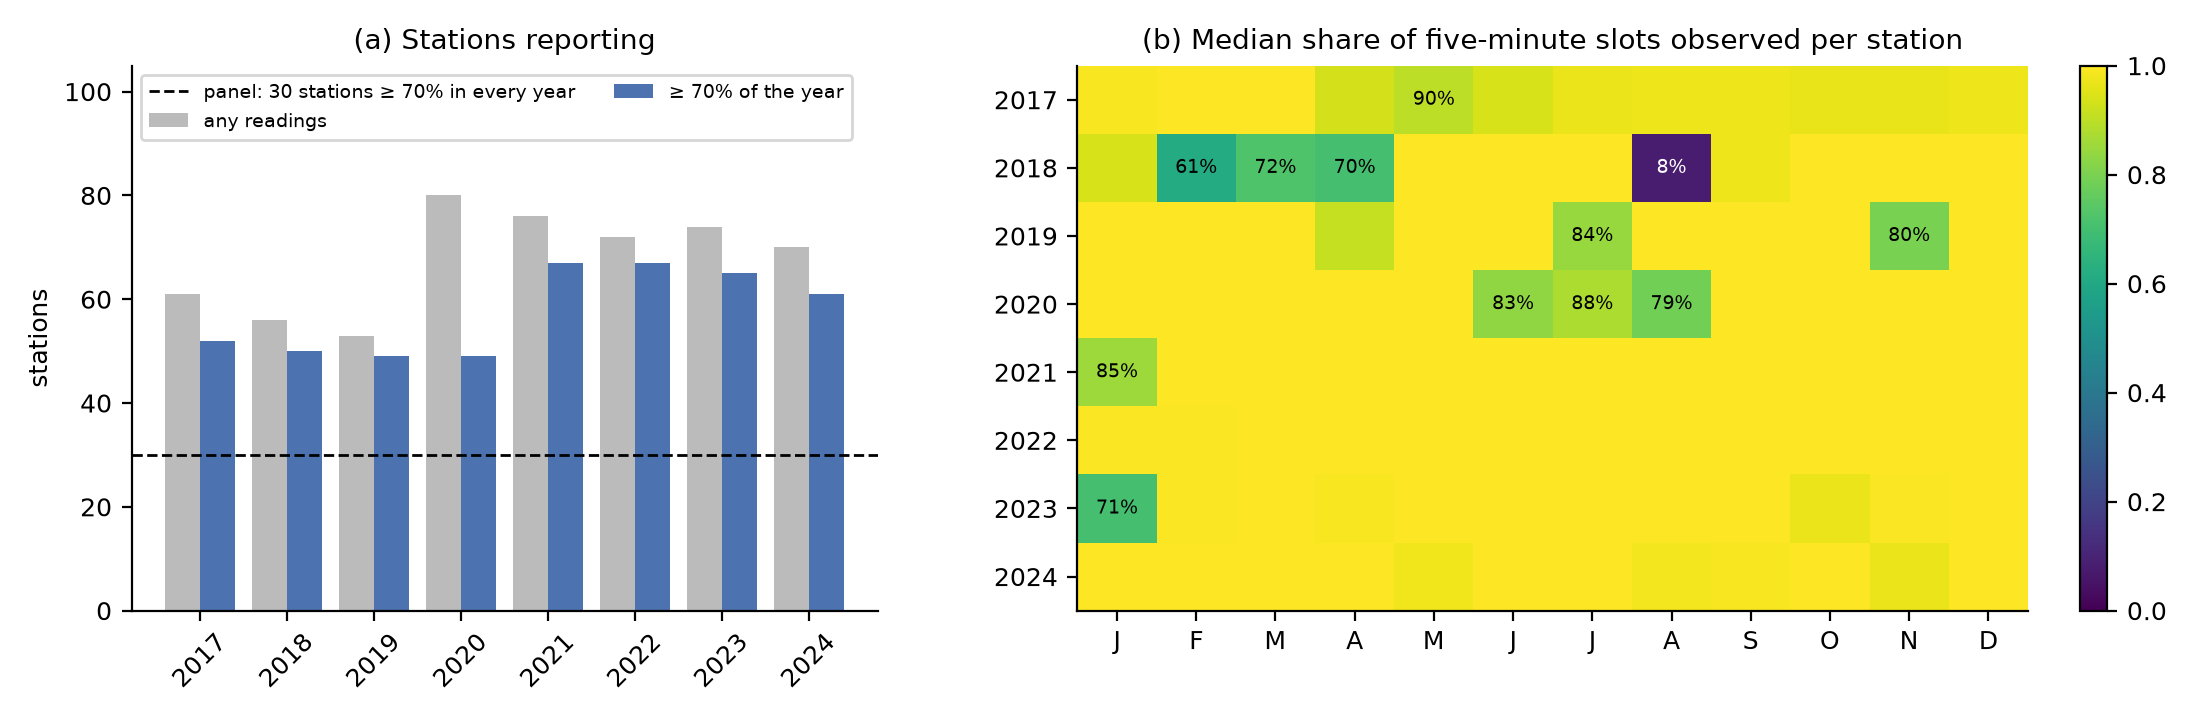
\includegraphics[width=\linewidth]{fig1_coverage.png}
\caption{Data coverage. (a) Stations reporting each year. (b) Median share of five-minute slots observed per station-month: 2018 has network-wide outages in Feb--Apr (the readings at :25 and :55 are missing in March) and in August.}\label{fig:coverage}
\end{figure}

\subsection{Within the year: two wet seasons with different kinds of rain}
The panel stations receive 2,628\mm{} a year on average. The annual cycle has two maxima (Fig.~\ref{fig:annual}a): November (316\mm) and December (263\mm), at the onset of the NE monsoon, and April (252\mm). February (136\mm) and July (151\mm) are the driest months. The same month often differs between years by a factor of two or more (dots in Fig.~\ref{fig:annual}a).

Splitting monthly rainfall into how often it rains (share of wet readings) and how hard (rain per wet reading) shows that the two wet seasons differ. \textbf{January has the most frequent rain} (4.3\% of readings) \textbf{but the weakest} (7.5\,mm/h): NE monsoon surges bring long, widespread spells, and events longer than six hours give 31\% of January's rain compared with 4--8\% in March--July (Fig.~\ref{fig:events}a). \textbf{March to May have the most intense rain} (11--12\,mm/h) and the shortest, most intense events (Fig.~\ref{fig:events}c): inter-monsoon thunderstorms.

\begin{figure}[H]
\centering
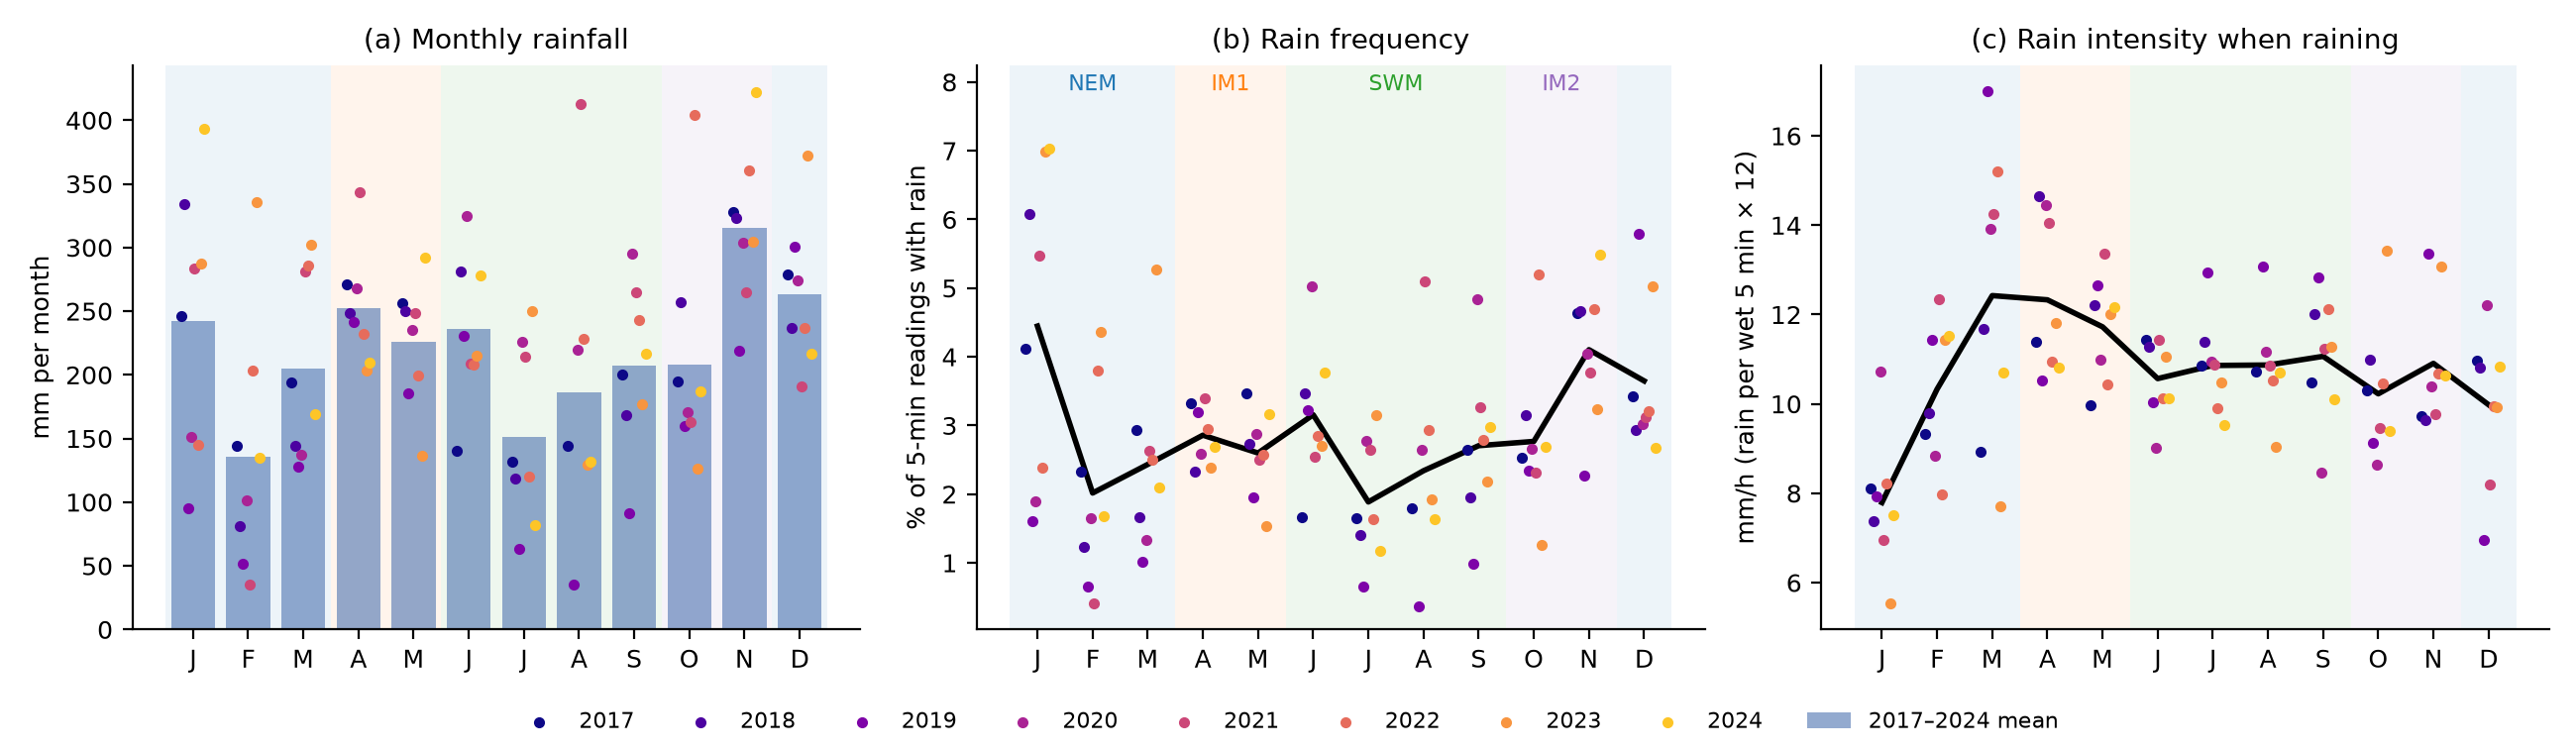
\includegraphics[width=\linewidth]{fig2_annual_cycle.png}
\caption{Annual cycle of the 30-station panel. (a) Monthly rainfall, 2017--2024 mean (bars) and individual years (dots). (b) Share of five-minute readings with rain. (c) Mean intensity of wet readings. Shading marks the four seasons.}\label{fig:annual}
\end{figure}

The \textbf{time of day} matters as much as the season (Fig.~\ref{fig:diurnal}). In the NE monsoon and both inter-monsoons, rain is concentrated in the afternoon: the mean rate peaks at 15--16\,h SGT at 2.5--3.7 times its daily mean, and the share of wet hours reaches 14--22\%, against 3--5\% at night. This is convection driven by daytime heating. The SW monsoon is different: its rate peaks at 09\,h with a flatter cycle (peak/mean 2.1), and rain-weighted event starts peak at 08\,h (Fig.~\ref{fig:events}b). This matches the pre-dawn and morning ``Sumatra squalls'', lines of storms that form over Sumatra and the Strait of Malacca and cross Singapore from the west \hyperref[ref:2]{[2]}.

\begin{figure}[H]
\centering
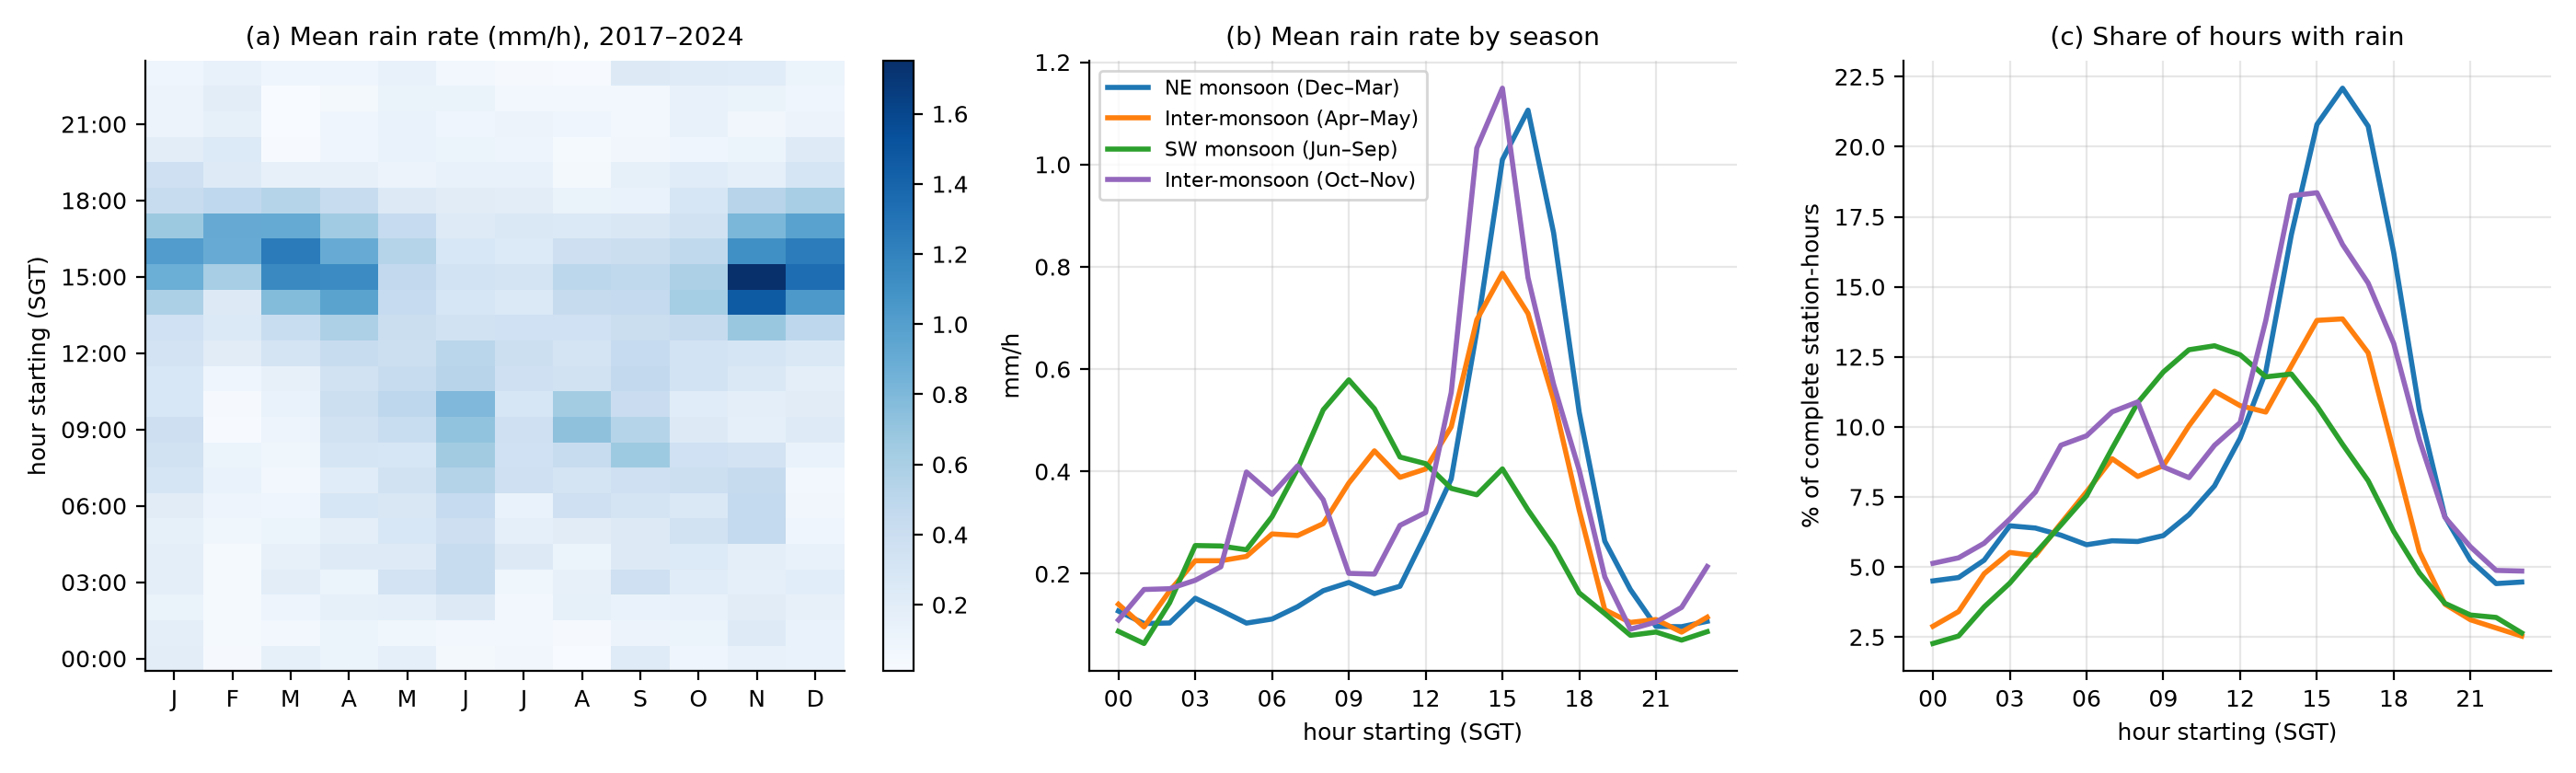
\includegraphics[width=\linewidth]{fig3_diurnal.png}
\caption{Diurnal cycle, all stations. (a) Mean rain rate by hour and month. (b) Mean rain rate by hour and season. (c) Share of fully observed station-hours with rain. A reading stamped $t$ is assigned to the hour containing $t-5$\,min.}\label{fig:diurnal}
\end{figure}

\begin{figure}[H]
\centering
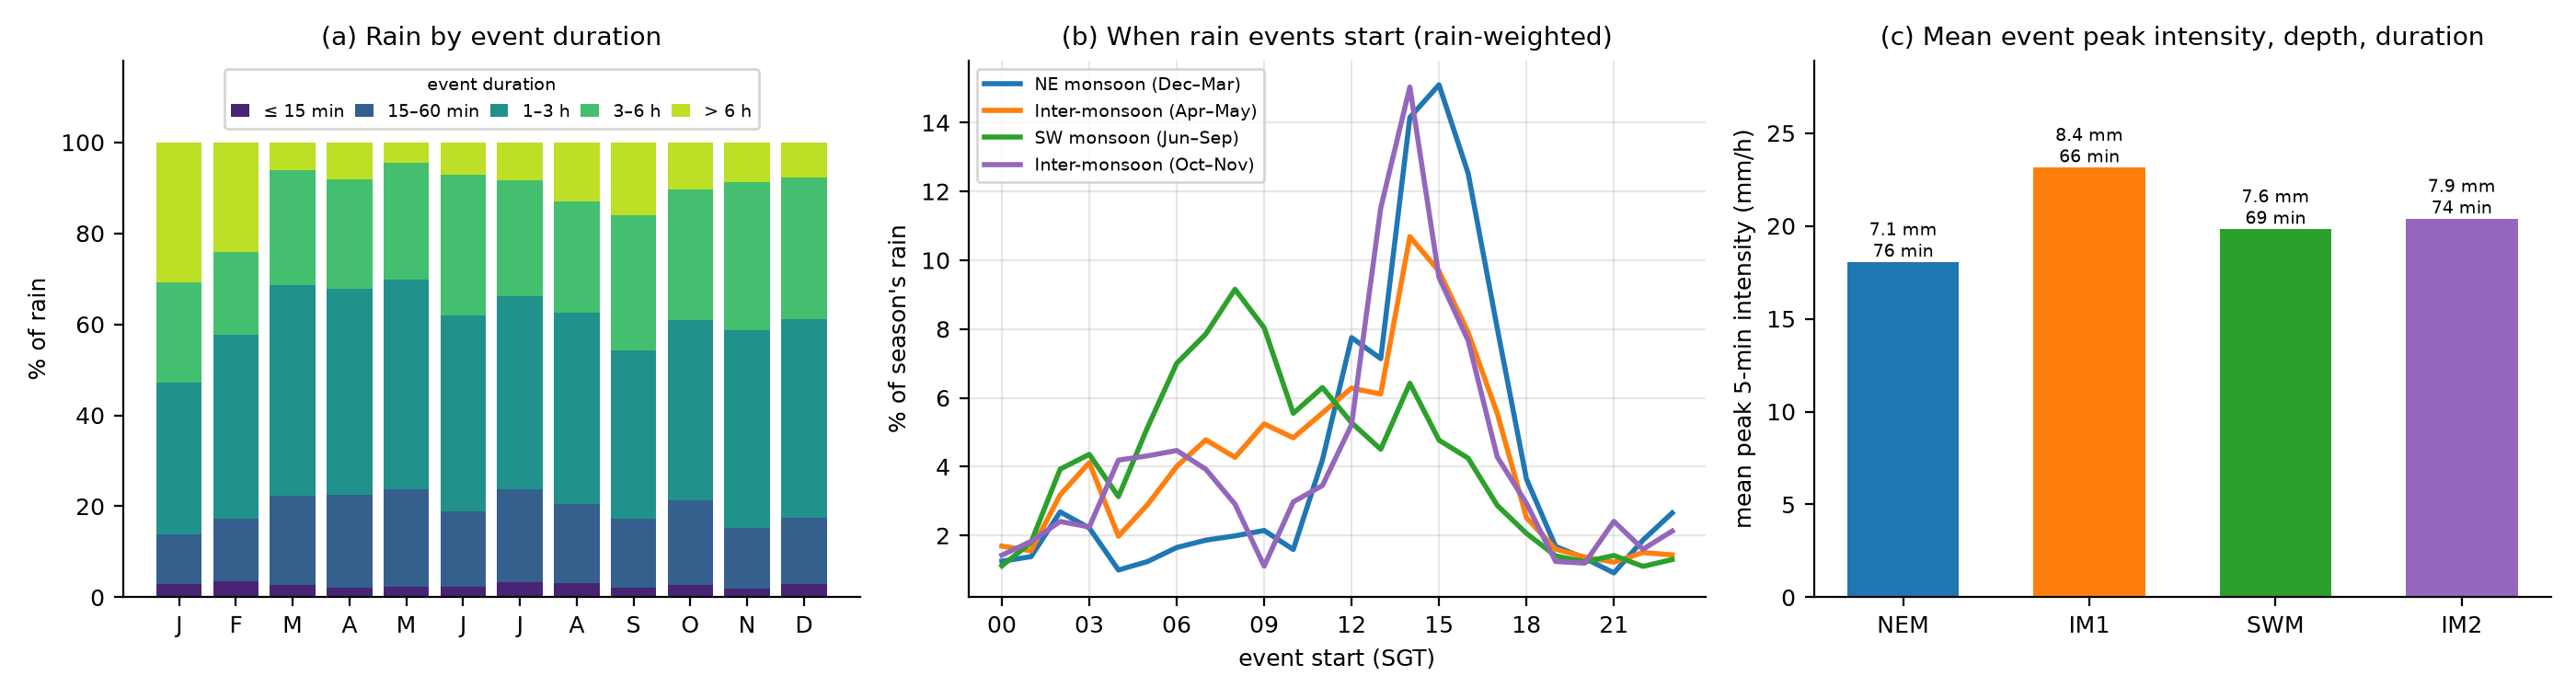
\includegraphics[width=\linewidth]{fig7_events.png}
\caption{Rain events (wet readings separated by at least one dry hour; 155,703 fully observed events). (a) Share of each month's rain by event duration. (b) Start hour of events, weighted by event depth. (c) Mean peak five-minute intensity, with mean depth and duration.}\label{fig:events}
\end{figure}

\subsection{Across the island: a west--east gradient that depends on the season}
Mean annual totals range from 1,733\mm{} in the east to 3,292\mm{} in the west (Fig.~\ref{fig:spatial}a). The rank correlation between a station's longitude and its total relative to the island mean is $-0.68$. The gradient is strongest in the SW monsoon ($-0.79$; Fig.~\ref{fig:spatial}d), when storms arrive from the west and weaken across the island. It is weakest in the NE monsoon ($-0.28$), when the north is wetter instead (correlation with latitude $+0.39$).

\begin{figure}[H]
\centering
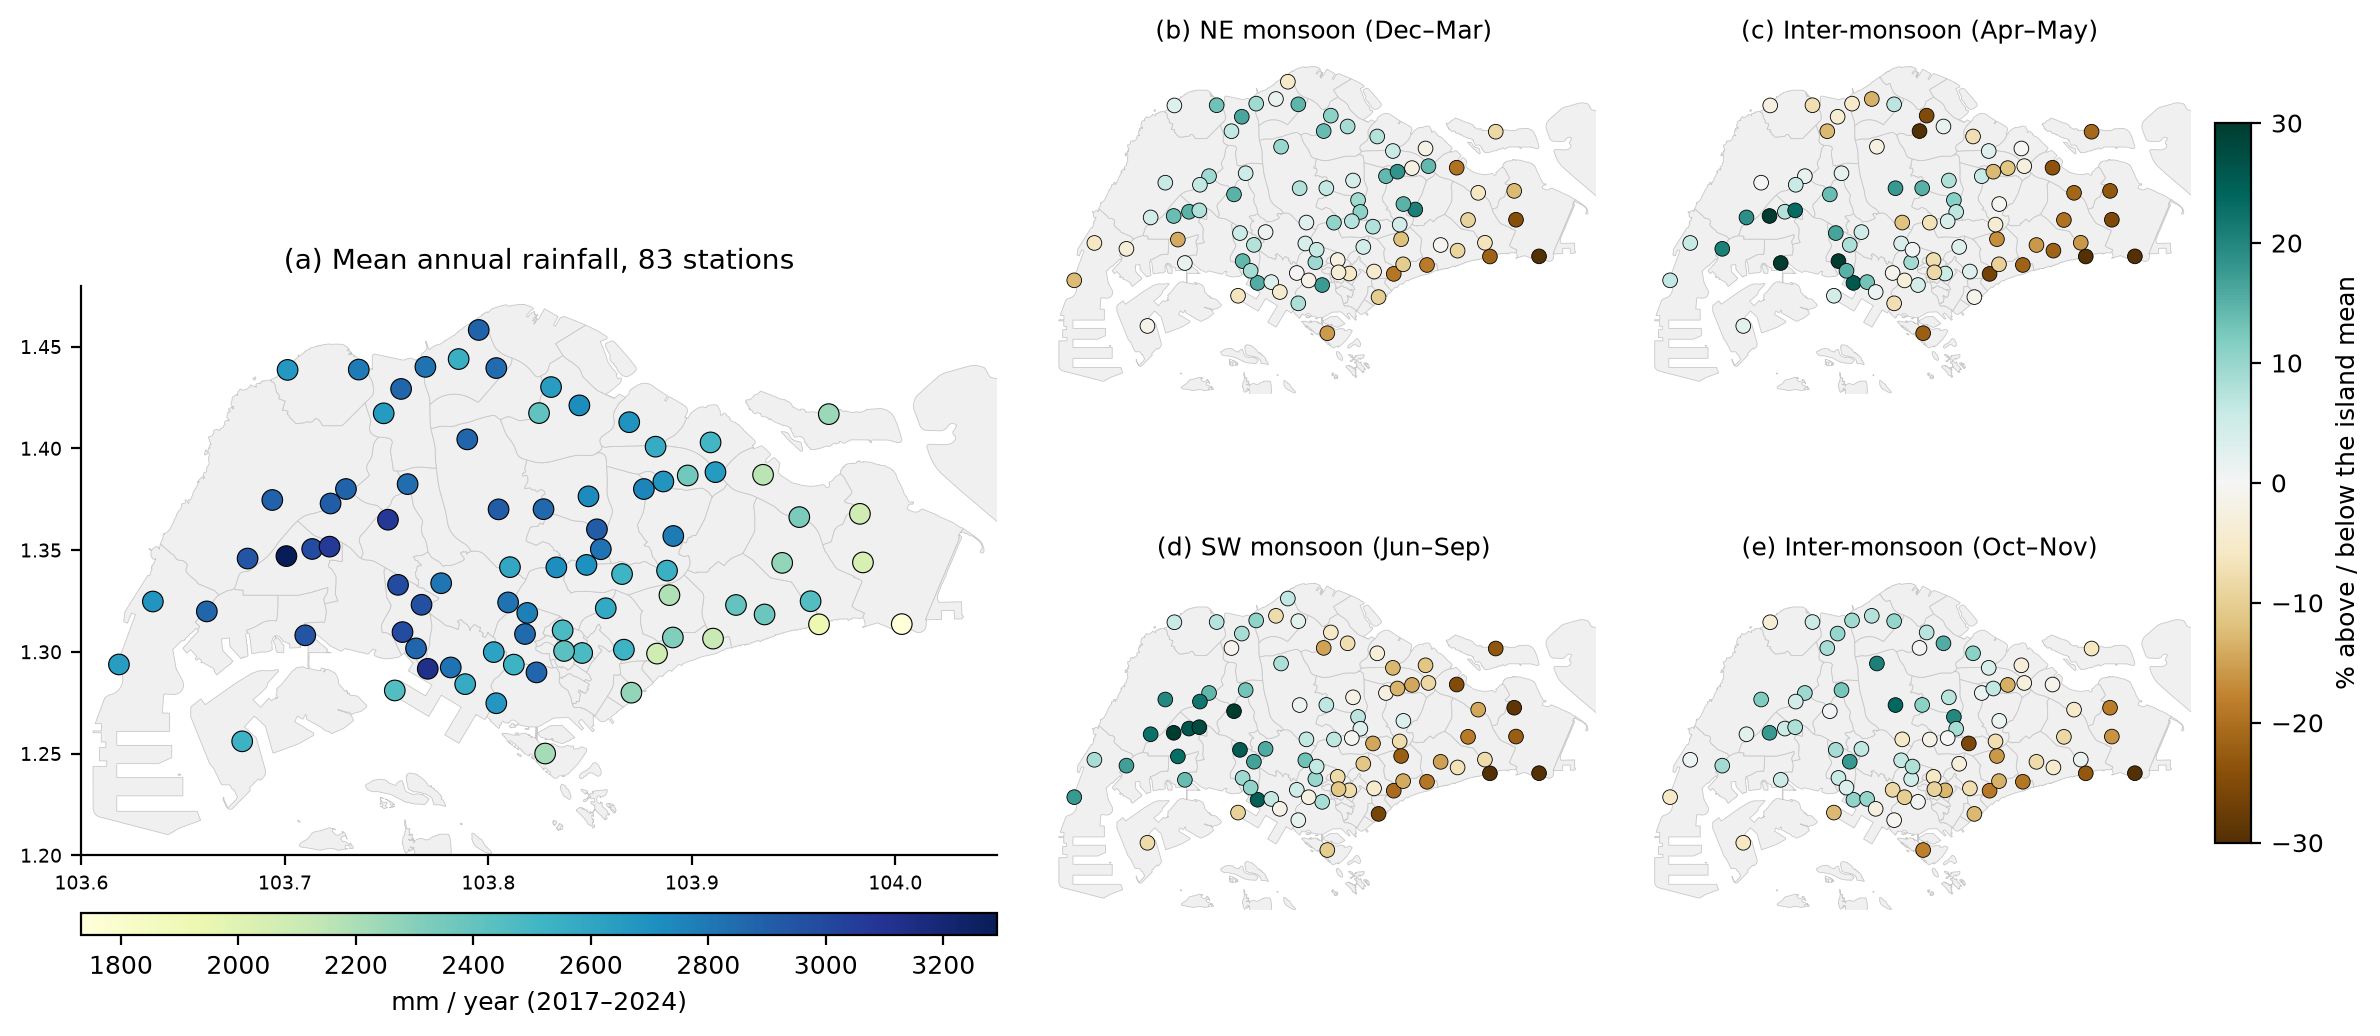
\includegraphics[width=\linewidth]{fig4_spatial.png}
\caption{Spatial pattern, 83 stations with enough data. (a) Mean annual rainfall. (b)--(e) Seasonal totals relative to the island mean over the same months, so stations with different reporting periods are comparable. Boundary: Master Plan 2019 planning areas \hyperref[ref:3]{[3]}.}\label{fig:spatial}
\end{figure}

How far rain extends is measured by the correlation between station pairs (Fig.~\ref{fig:corr}). For hourly totals the correlation falls to $1/e$ at 14--17\,km in every season: an hour of rain is a local event. Daily totals are coherent over longer distances, most in the NE monsoon (39\,km, organised monsoon rain) and least in IM1 (26\,km, isolated thunderstorms).

\begin{figure}[H]
\centering
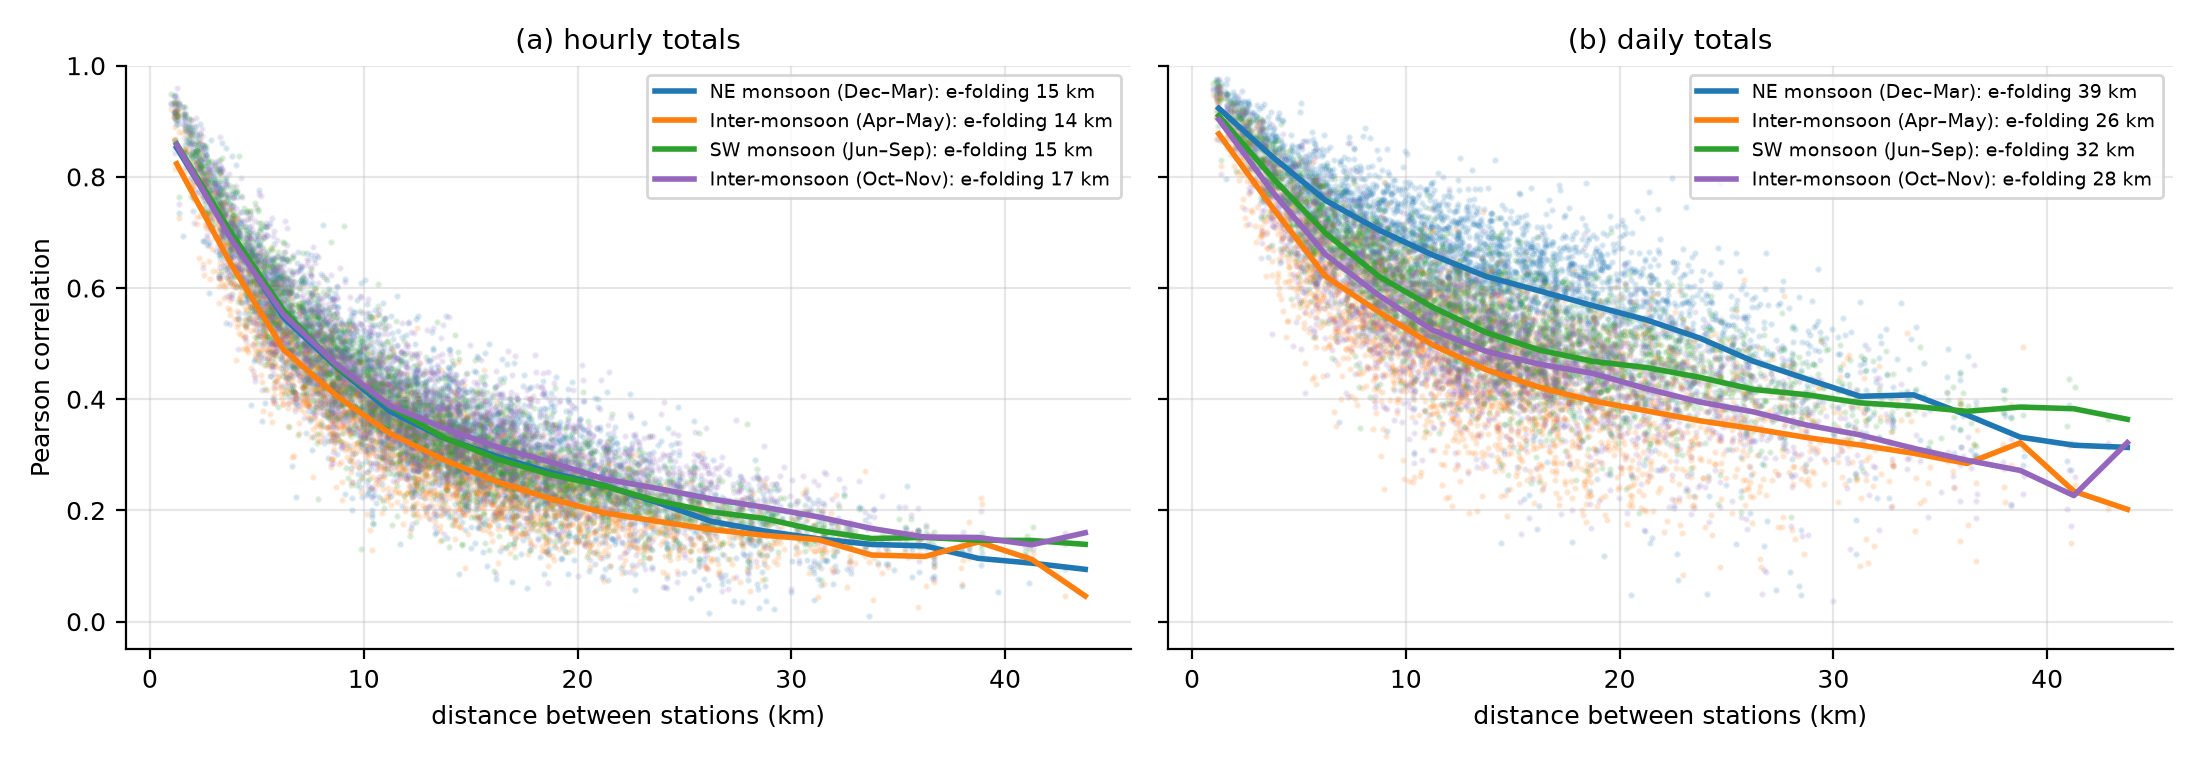
\includegraphics[width=\linewidth]{fig8_spatial_correlation.png}
\caption{Correlation between station pairs against distance, by season, for (a) fully observed hours and (b) days with at least 95\% of slots observed. Lines are binned means; the legend gives the e-folding distance $L$ of a fit $c_0 e^{-d/L}$.}\label{fig:corr}
\end{figure}

\subsection{Across years: dry years have fewer rain spells, not weaker ones}
Annual panel totals range from 1,803\mm{} in 2019, 31\% below the 2017--2024 mean, to 2,913\mm{} in 2021 (Fig.~\ref{fig:interannual}a); every year from 2020 to 2024 is above the mean. Individual months deviate far more: February 2023 had $+147\%$, August 2021 $+122\%$ and October 2022 $+94\%$, while August 2019 had $-81\%$ and February 2021 $-74\%$ (Fig.~\ref{fig:interannual}b).

Fig.~\ref{fig:freq}a decomposes each annual total into frequency and intensity. Annual totals correlate 0.98 with the share of wet readings and only 0.33 with the intensity of wet readings. In 2019 frequency was 31\% below average while intensity was within 2\%. \textbf{Dry years are years with fewer rain spells, not weaker storms.} Extremes vary less: the median annual maximum hourly rainfall per station stays between 54 and 63\mm, and hours above 20\mm{} range from 18 per station-year in 2019 to 32 in 2021 (Fig.~\ref{fig:freq}b,c).

\begin{figure}[H]
\centering
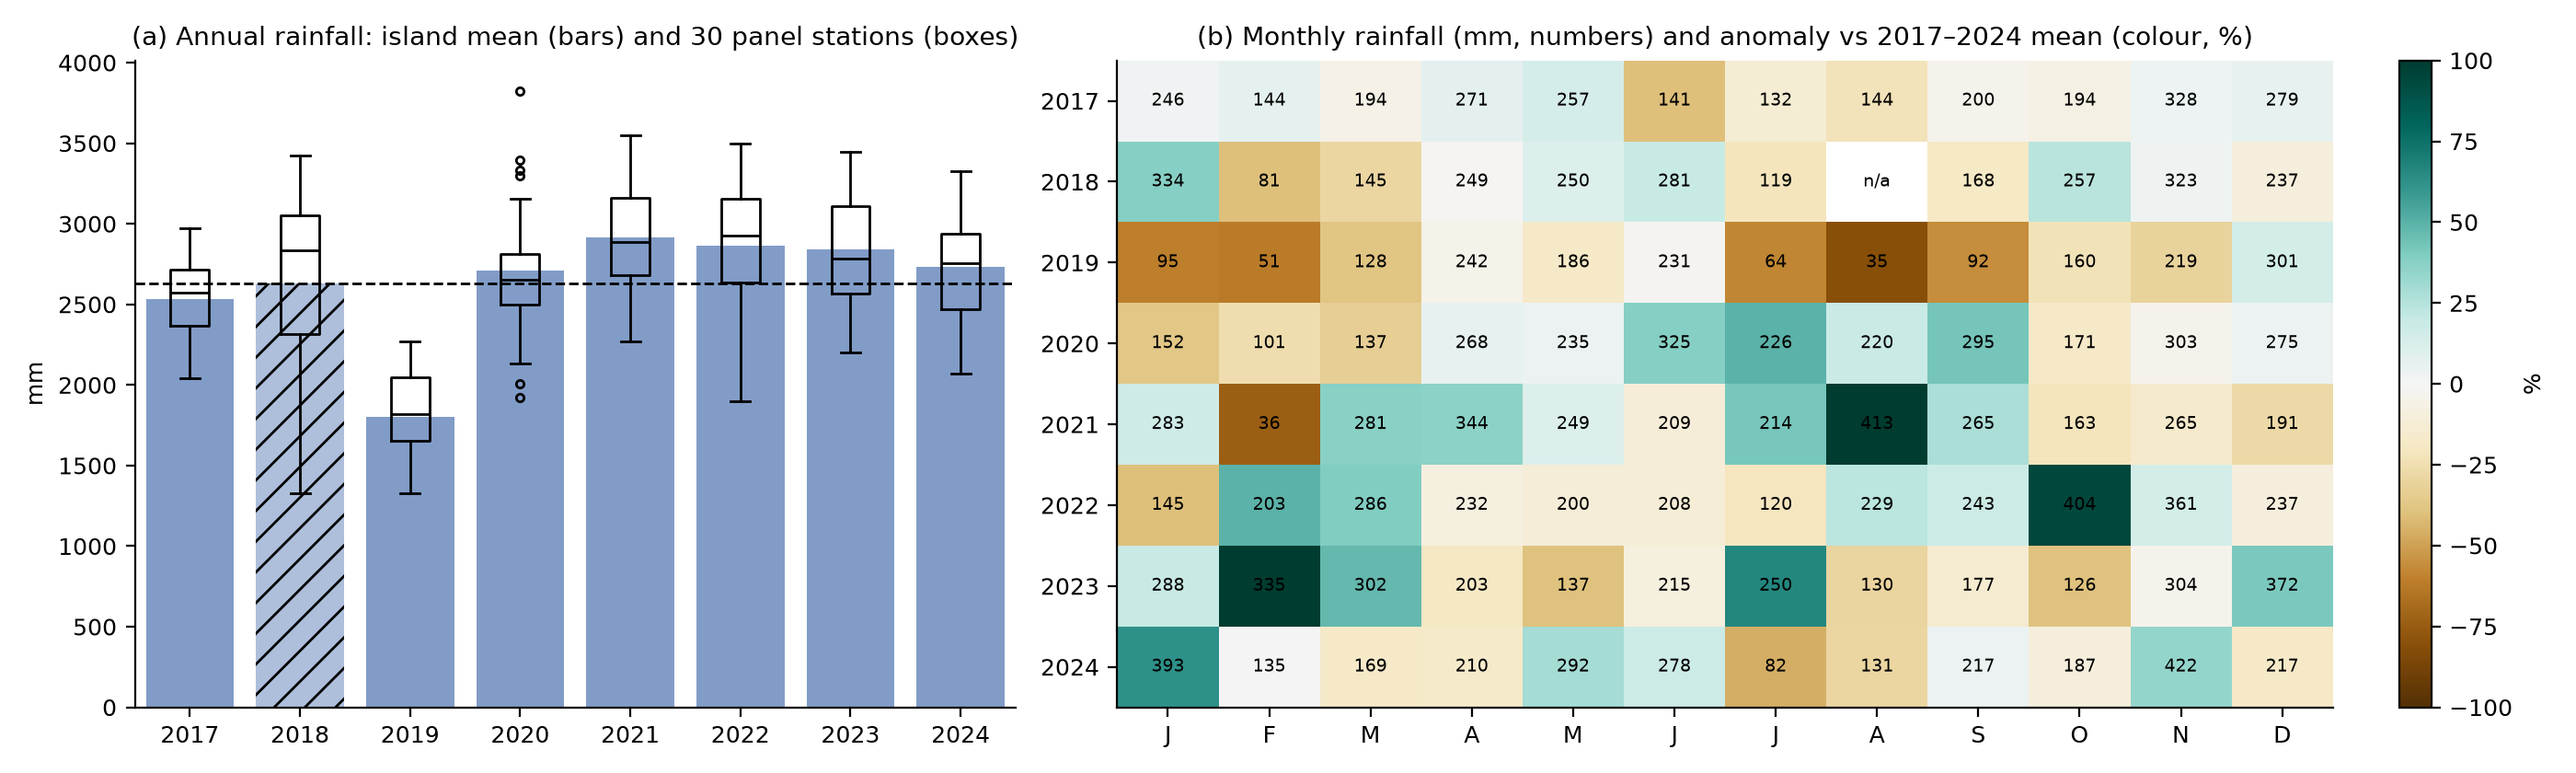
\includegraphics[width=\linewidth]{fig5_interannual.png}
\caption{Year-to-year variation. (a) Annual rainfall: panel mean (bars; 2018 hatched because August is imputed) and the 30 panel stations (boxes). (b) Monthly panel rainfall (numbers) and its anomaly against the 2017--2024 mean of the month (colour).}\label{fig:interannual}
\end{figure}

\begin{figure}[H]
\centering
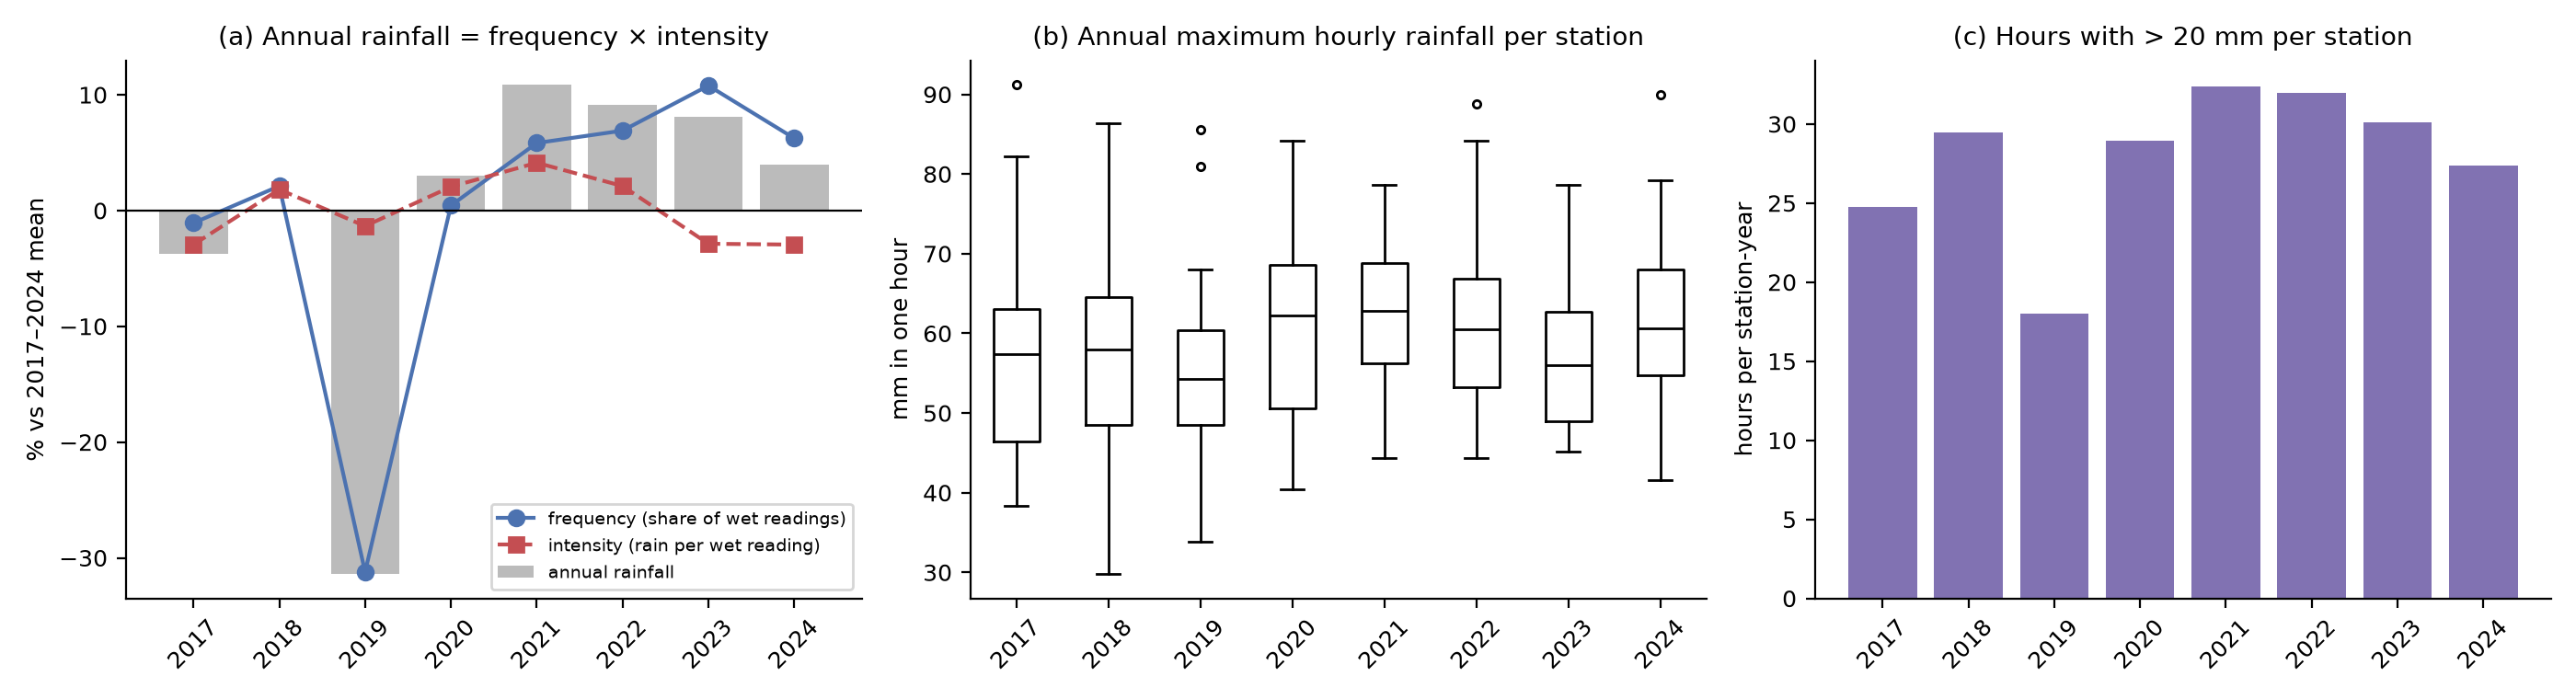
\includegraphics[width=\linewidth]{fig6_frequency_extremes.png}
\caption{(a) Annual rainfall, frequency and intensity as \% deviations from their 2017--2024 means. (b) Annual maximum hourly rainfall per station. (c) Hours above 20\mm{} per station-year, normalised by coverage.}\label{fig:freq}
\end{figure}

Kendall's test finds no trend in annual totals ($\tau=0.43$, $p=0.18$), intensity ($p=0.90$) or extremes ($p=0.55$). Wet frequency has $\tau=0.64$, $p=0.03$, but eight years cannot separate a trend from year-to-year variability. The pattern, a dry 2019 followed by wet years from 2020, is consistent with the strong positive Indian Ocean Dipole of 2019 and the La Niña years of 2020--2022, but we did not test this link. The spatial pattern also changes between years: in February--April 2018 every eastern station (longitude $>103.9^\circ$) received about 0.3 times the island mean while western stations received 1.2--2.1 times. Because all eastern gauges fell together, this was real rainfall rather than gauge faults, and it doubled the spread between stations that year (coefficient of variation 0.20 against 0.11--0.15).

\subsection{What this means for 30-minute forecasting}\label{sec:persist}
Fig.~\ref{fig:persist} links Task~1 to Task~2. \textbf{Persistence dominates}: after more than 5\mm{} in the last 30 minutes, the chance of more than 1\mm{} in the next 30 is 0.64; after a dry half-hour it is 0.0077, against 0.024 overall. In the dry state the probability follows the diurnal cycle, from about 0.002 at night to 0.02 at 14--15\,h. Rain is correlated only over about 15\,km at the hourly scale. These three facts motivate the feature groups of Section~\ref{sec:features}: recent rain at the station, rain at nearby stations, and the time of day and year.

\begin{figure}[H]
\centering
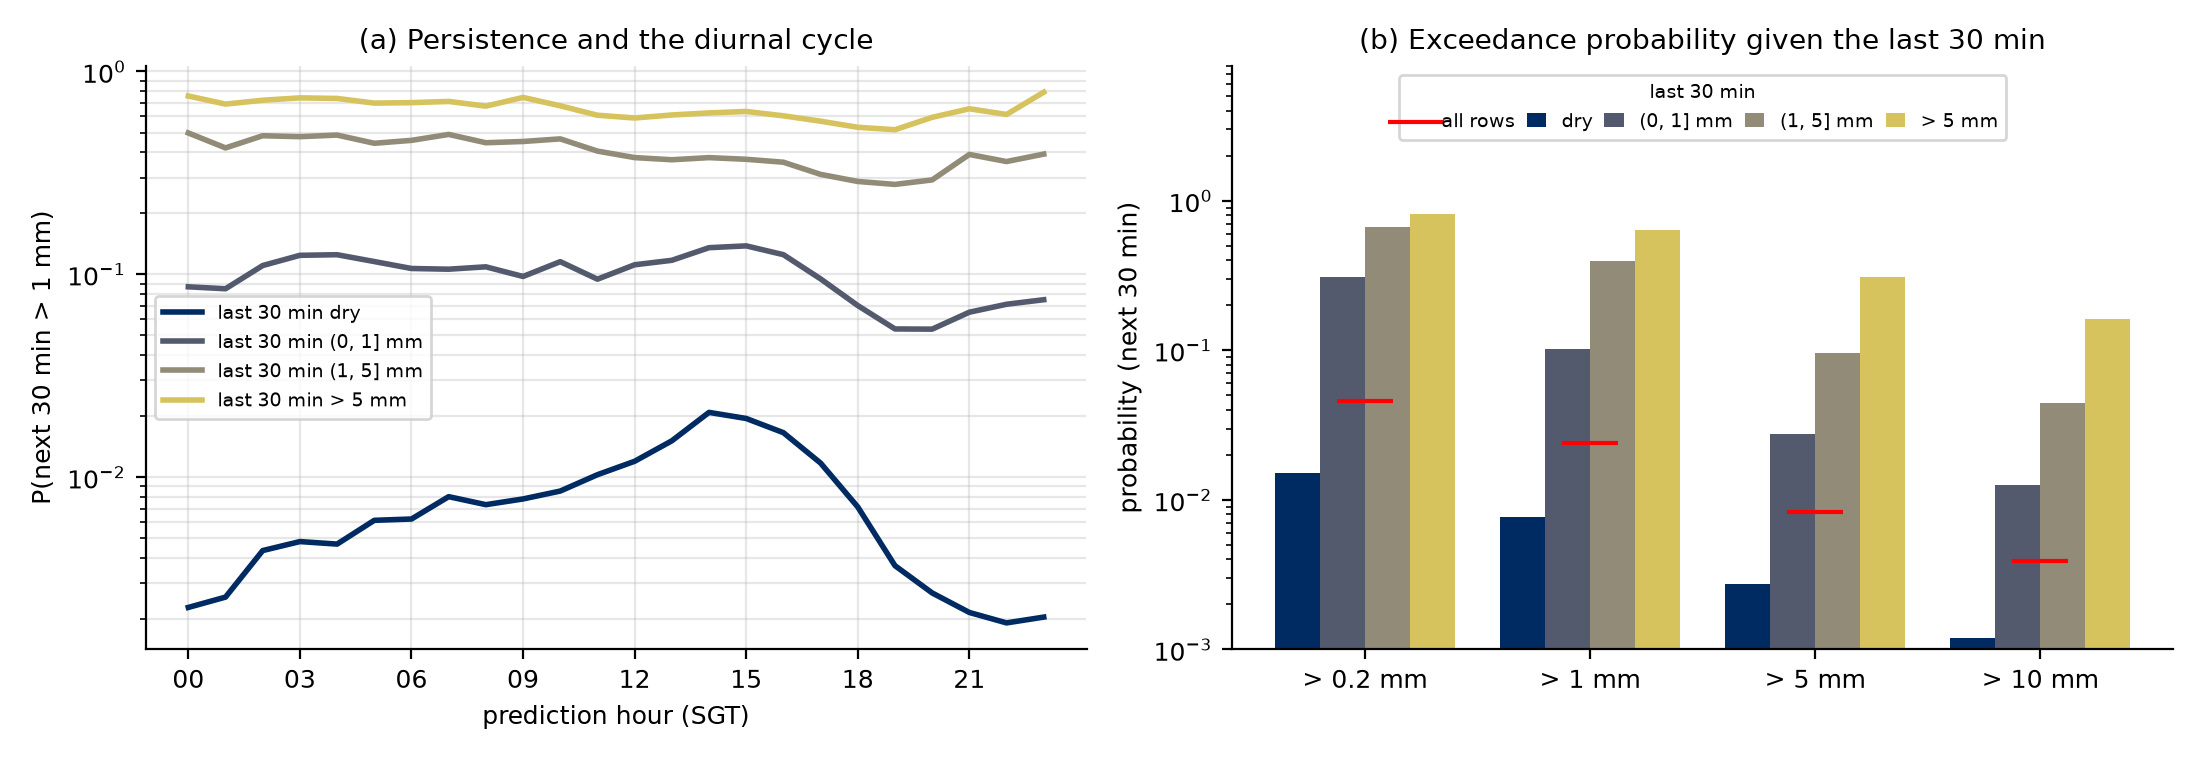
\includegraphics[width=\linewidth]{fig9_persistence.png}
\caption{Persistence in the eligible 2017--2024 rows. (a) $P(\text{next 30 min} > 1\text{\mm})$ by hour and by rain in the last 30 minutes. (b) Exceedance probabilities by rain in the last 30 minutes; red bars are the overall rates.}\label{fig:persist}
\end{figure}

\section{Task 2: problem set-up and feature selection}\label{sec:features}
\subsection{Prediction problem and data split}
A row is a (station, five-minute slot) pair. Its target $Y$ is the total of the six readings after the prediction time; its features use only readings at or before that time. The label for a threshold $r$ is $\mathbb{1}\{Y > r\}$, created when the model is queried. Years are split in time: \textbf{2017--2022 for training} (33.7\,M eligible rows after QC, of which 2.04\,M are wet), \textbf{2023 for validation} (6.7\,M) and \textbf{2024 for testing} (6.3\,M). Every model choice in this report was made by a rule on 2023. Events are rare: in 2024, 2.6\% of rows exceed 1\mm{} and 0.10\% exceed 20\mm.

\subsection{Features}
Table~\ref{tab:features} lists the 69 features of the final model. They were added in two stages, each kept because it improved a 2023 validation score. Neighbour aggregates raised the 2023 PR-AUC of the 1\mm{} GBT baseline from 0.568 to 0.615. The slot-exact, per-neighbour and storm features then lowered the 2023 lattice log-loss of the Gaussian ZILN model (Section~\ref{sec:ziln}) from 0.3093 to 0.2991.

\begin{table}[H]
\centering\small
\caption{Features of the final model. Neighbour values come from the slot before the prediction time, so no neighbour reading is newer than the station's own latest reading, even when exports disagree by one second.}\label{tab:features}
\renewcommand{\arraystretch}{1.15}
\begin{tabularx}{\linewidth}{@{}p{0.22\linewidth}Yr@{}}
\toprule
\textbf{Group} & \textbf{Features} & \textbf{n} \\
\midrule
Station & station index (fitted on training years), longitude, latitude & 3 \\
Own recent rain & rain in the last 5/15/30/60 min; current and two lagged readings; 15/30/60-min and 3-h sums on exact slots; 60-min peak; 3-h completeness & 13 \\
Neighbour aggregates & number, weight and nearest distance of reporting neighbours; inverse-distance mean of their 5/15/30/60-min rain; their maximum 30-min rain; share raining & 9 \\
Individual neighbours & for each of the 8 nearest stations: latest reading, 15-min sum, availability & 24 \\
Storm geometry & maximum 60-min and inverse-distance 3-h neighbour rain; distance to the nearest wet neighbour; rain-weighted centroid of neighbour rain now and 15 min earlier, its displacement and radial approach & 11 \\
Calendar & hour and month (sine, cosine), day of week, minute of day and day of year (sine, cosine) & 9 \\
\bottomrule
\end{tabularx}
\end{table}

Each group answers a finding of Task~1. Own recent rain captures persistence at several time scales. The eight nearest neighbours are a median 3.9\,km away and 97\% lie within 10\,km, well inside the 15\,km over which hourly rain is correlated; the storm-centroid features follow rain that moves across the network, such as the SW-monsoon squalls arriving from the west. Calendar features carry the diurnal and seasonal cycles, and the station index and coordinates carry the west--east gradient. A missing neighbour is never read as zero rain: aggregates use only reporting neighbours, and availability features mark the rest. In the occurrence GBT, neighbour rain takes most of the split gain: the inverse-distance mean of neighbours' last five minutes (0.28), the distance to the nearest wet neighbour (0.14) and the maximum 60-minute neighbour rain (0.12), followed by the station index (0.06) and the station's own recent rain (0.04 for the 5-minute sum, 0.03 for the current reading). In the GBT for the log-amount $m(x)$, the station's current reading (0.21) and the station index (0.15) lead. Correlated features share gain, so these figures rank groups only roughly.

\section{Task 2: model development}\label{sec:model}
\subsection{Baselines: one classifier per threshold}\label{sec:baselines}
The first models were standard Spark classifiers for the single threshold $r=1$\mm: logistic regression, random forest, GBT and a multilayer perceptron. They used the station and neighbour aggregate features, a 3:1 subsample of negative rows and inverse-frequency class weights, with the F1-optimal probability cut-off chosen on 2023. The GBT discriminated best (Table~\ref{tab:compare}), and the MLP failed to train (2023 ROC-AUC 0.46). Two problems remained. First, resampling distorts the output: the GBT scores have a Brier skill score of $-2.05$ on 2024, so they are not probabilities until recalibrated (Platt scaling \hyperref[ref:8]{[8]} fitted on 2023 gives 0.385). Second, the task needs any threshold, and one classifier per threshold cannot guarantee that $P(Y>r)$ falls as $r$ rises.

\subsection{One model for every threshold}\label{sec:ziln}
We therefore model the whole distribution of $Y$. Writing $\pi(x) = P(Y>0\mid x)$ and $S(r\mid x) = P(Y>r \mid Y>0, x)$,
\[
P(Y > r \mid x) = \pi(x)\, S(r \mid x),
\]
which is monotone in $r$ by construction and answers every threshold from one fitted model.

\textbf{Zero-inflated lognormal (ZILN) \hyperref[ref:5]{[5]}.} Here $\log Y \mid Y>0, x \sim \mathcal N\big(m(x), s(x)^2\big)$. The likelihood separates, so each part is a maximum-likelihood fit with a Spark MLlib estimator \hyperref[ref:4]{[4]}:
\begin{itemize}[leftmargin=1.5em,itemsep=3pt]
\item $\pi$: \texttt{GBTClassifier} on $\mathbb 1\{Y>0\}$. Dry rows are subsampled at rate $q=0.19$ and weighted $1/q$, which keeps the log loss unbiased and the probabilities calibrated.
\item $m$: \texttt{GBTRegressor} on $\log Y$ over wet rows.
\item $s^2$: \texttt{GBTRegressor} on cross-fitted squared residuals (two folds, so no row's residual comes from a model that saw it), or a constant.
\end{itemize}
Tipping-bucket totals pile up at one tip (0.2\mm), so the standardised residuals are skewed. Besides the Gaussian, we therefore tried their empirical distribution, globally and per decile of $m(x)$. 2023 chose the GBT variance with residual distributions per decile, which corrects an underestimate of $P(Y>5\text{\mm})$ of about 17\% under the Gaussian. A non-Spark prototype, used only to choose the family, preferred the ZILN to Bernoulli--Gamma and Tweedie distributions on 2023 (lattice log-loss 0.298 against 0.306 and 0.309).

\textbf{Nonparametric amount models.} A continuous distribution cannot represent the atom at a single tip: ZILN over-predicts $P(Y>0.2\text{\mm})$ by 15\%. We kept $\pi(x)$ and the assembled features and replaced $S$ by estimates on the grid of edges 0.2, 0.4, 0.5, 1, 1.4, 2, 3, 5, 7, 10, 15, 20, 30 and 50\mm, all trained with Spark MLlib on the 2.04\,M wet training rows:
\begin{itemize}[leftmargin=1.5em,itemsep=3pt]
\item \textbf{hazard}: a \texttt{GBTClassifier} on one row per edge a wet total reaches (a continuation-ratio model), so $S$ is a product of conditional probabilities;
\item \textbf{rf}: a \texttt{RandomForestClassifier} over the 15 wet classes;
\item \textbf{mlp}: a \texttt{MultilayerPerceptronClassifier} (two hidden layers of 64 units, softmax over the 15 classes, L-BFGS) on asinh-transformed, standardised features with the station one-hot encoded.
\end{itemize}
For rf and mlp, $S(e_j\mid x)$ is the summed probability of the classes above edge $e_j$. Between edges the prediction interpolates linearly in $(\log r, \log P)$, and beyond 50\mm{} it extends the last segment as a Pareto tail, so any $r\ge0$ has a probability.

\subsection{Model selection}
Every candidate, and equal-weight mixtures of ZILN with them, was turned into the same grid forecast on identical rows. The pre-declared rule picks the single model with the \textbf{lowest 2023 log score over the grid classes}, a strictly proper score of the whole forecast distribution \hyperref[ref:6]{[6]}. Table~\ref{tab:candidates} shows that the MLP wins on 2023 and keeps the same ranking in 2024. Uncertainty comes from a bootstrap of 2,000 replicates over the 366 days of 2024, since rows within a day are strongly dependent \hyperref[ref:7]{[7]}.

\begin{table}[H]
\centering\small
\caption{Amount-model candidates (original data, ZILN occurrence model). Log score and CRPS (grid approximation on [0, 50]\mm): lower is better. BSS: Brier skill score against the 2017--2022 climatology. P/O: mean forecast over event rate.}\label{tab:candidates}
\renewcommand{\arraystretch}{1.15}
\begin{tabular*}{\linewidth}{@{\extracolsep{\fill}}lcccccccc@{}}
\toprule
& \multicolumn{2}{c}{\textbf{Log score}} & \textbf{CRPS} & \multicolumn{3}{c}{\textbf{BSS 2024}} & \multicolumn{2}{c}{\textbf{P/O 2024}} \\
\cmidrule(lr){2-3}\cmidrule(lr){5-7}\cmidrule(lr){8-9}
\textbf{Model} & 2023 & 2024 & 2024 & 1\mm & 5\mm & 20\mm & 0.2\mm & 20\mm \\
\midrule
ZILN & .2492 & .2465 & .1027 & .443 & .298 & .104 & 1.15 & 1.33 \\
hazard & .2331 & .2306 & .1018 & .442 & .299 & .123 & 1.02 & 0.96 \\
rf & .2344 & .2320 & .1027 & .441 & .291 & .115 & 1.01 & 1.10 \\
\textbf{mlp (selected)} & \textbf{.2319} & \textbf{.2293} & .1012 & \textbf{.451} & .305 & .120 & 1.03 & 1.11 \\
ZILN+hazard+rf+mlp & .2335 & .2308 & \textbf{.1010} & .449 & \textbf{.306} & \textbf{.127} & 1.05 & 1.13 \\
\bottomrule
\end{tabular*}
\end{table}

\textbf{Final model:} the occurrence GBT of the ZILN model and the MLP amount model, both refitted on the QC'd training data and saved in \path{models/ziln_rich_qc} and \path{models/amount_mlp_qc}. Table~\ref{tab:hyper} gives their settings.

\begin{table}[H]
\centering\small
\caption{Settings of the final model (Spark MLlib). For the GBTs, 2023 chose this configuration over 60 trees with step 0.05 (lattice log-loss 0.3093 against 0.3174).}\label{tab:hyper}
\renewcommand{\arraystretch}{1.15}
\begin{tabularx}{\linewidth}{@{}p{0.27\linewidth}Y@{}}
\toprule
Occurrence $\pi$ & \texttt{GBTClassifier}: 120 trees, depth 6, step 0.2, 128 bins, subsampling 0.8; dry rows kept at $q=0.193$ with weight $1/q$ \\
Amount $S$ & \texttt{MultilayerPerceptronClassifier}: layers 155--64--64--15 (68 asinh-transformed numeric features + 87-station one-hot), L-BFGS, 300 iterations, block size 1024; \texttt{StandardScaler} fitted on training rows \\
ZILN amount part (baseline) & \texttt{GBTRegressor} for $m$ and $\log s^2$: 100 trees, depth 6, step 0.1; residual distribution per decile of $m$ \\
\bottomrule
\end{tabularx}
\end{table}

The prediction script takes the three inputs of the task:
\begin{lstlisting}[basicstyle=\footnotesize\ttfamily]
python scripts/predict_rain_probability.py --station S50 --time 2024-11-03T15:00 \
    --threshold 0.2 1 5 20
# station S50 at 2024-11-03 15:00:00 (SGT): P(any rain in next 30 min) = 0.0357
#   P(rainfall > 0.2 mm in next 30 min) = 0.0214
#   P(rainfall > 1 mm in next 30 min) = 0.0121
#   P(rainfall > 5 mm in next 30 min) = 0.0043
#   P(rainfall > 20 mm in next 30 min) = 0.0004
\end{lstlisting}

\section{Task 2: results}\label{sec:results}
\subsection{Comparison with the baselines}
Table~\ref{tab:compare} compares all models at $r=1$\mm{} on the same 6,334,889 eligible rows of the original (not QC'd) 2024 data. The threshold-free models discriminate better than the best single-threshold classifier (PR-AUC 0.649 against 0.605) and are calibrated without any post-processing; the final model's Brier skill score of 0.450 compares with 0.385 for the Platt-calibrated GBT. Training on the QC'd data leaves the scores unchanged within 0.001.

\begin{table}[H]
\centering\small
\caption{All models at $r=1$\mm, original 2024 data (6,334,889 rows, 2.57\% events). F1 uses the cut-off that maximises F1 on 2023. BSS of the baselines uses the 2024 event rate as reference; ours uses the 2017--2022 rate (the difference is below 0.001).}\label{tab:compare}
\renewcommand{\arraystretch}{1.15}
\begin{tabular*}{\linewidth}{@{\extracolsep{\fill}}lcccc@{}}
\toprule
\textbf{Model} & \textbf{ROC-AUC} & \textbf{PR-AUC} & \textbf{BSS} & \textbf{F1} \\
\midrule
Persistence rule (last 30 min $>1$\mm) & -- & -- & -- & .516 \\
Logistic regression, station features & .878 & .457 & $-4.14$ (uncalibrated) & .514 \\
GBT, station + neighbour aggregates & .935 & .605 & $-2.05$ / .385 (Platt) & .594 \\
ZILN, 69 features & .939 & .641 & .443 & .610 \\
ZILN occurrence + MLP amount & .940 & .649 & .451 & .616 \\
\textbf{Final model (same, trained on QC'd data)} & \FinalOrigROC & \FinalOrigPR & \FinalOrigBSS & \FinalOrigFone \\
\bottomrule
\end{tabular*}
\end{table}

\subsection{All thresholds}
Table~\ref{tab:final} and Fig.~\ref{fig:skill}a report the final model on the QC'd 2024 rows, against a ZILN model fitted to the same data. Skill falls with the threshold because heavy 30-minute totals are rarer and harder to anticipate, from 0.52 at 0.2\mm{} to 0.12 at 20\mm; ROC-AUC stays at 0.94--0.96 throughout. The final model is better than ZILN at every threshold, and every bootstrap interval of the gain excludes zero; the largest gain is at 0.2\mm, where it removes ZILN's 15\% over-prediction. The reliability diagram (Fig.~\ref{fig:skill}b) follows the diagonal over three orders of magnitude at every threshold; only the lowest bins over-predict (at 1\mm, forecasts of 0.0016 for an observed 0.0011). At 1\mm{} the mean forecast is within 1\% of the event rate.

\begin{table}[H]
\centering\small
\caption{Final model on QC'd 2024 (6,298,383 rows). Gain: Brier-skill gain over ZILN fitted to the same data, with day-block bootstrap 95\% interval. F1 cut-offs chosen on 2023.}\label{tab:final}
\renewcommand{\arraystretch}{1.15}
\begin{tabular*}{\linewidth}{@{\extracolsep{\fill}}lccccccc@{}}
\toprule
$r$ (mm) & 0.2 & 0.5 & 1 & 2 & 5 & 10 & 20 \\
\midrule
Event rate & .049 & .037 & .026 & .017 & .0084 & .0038 & .0010 \\
ROC-AUC & .939 & .941 & .940 & .938 & .940 & .948 & .965 \\
PR-AUC & .730 & .699 & .649 & .575 & .461 & .338 & .159 \\
F1 & .674 & .651 & .616 & .561 & .483 & .409 & .284 \\
BSS, ZILN & .496 & .487 & .442 & .379 & .298 & .219 & .106 \\
\textbf{BSS, final} & \textbf{.517} & \textbf{.493} & \textbf{.451} & \textbf{.389} & \textbf{.306} & \textbf{.228} & \textbf{.119} \\
\multirow{2}{*}{Gain} & +.021 & +.006 & +.009 & +.010 & +.008 & +.010 & +.013 \\
& {\scriptsize[.017,.026]} & {\scriptsize[.003,.008]} & {\scriptsize[.004,.014]} & {\scriptsize[.004,.019]} & {\scriptsize[.004,.012]} & {\scriptsize[.004,.014]} & {\scriptsize[.007,.018]} \\
Mean forecast / rate & 1.03 & 1.01 & 1.01 & 1.02 & 1.04 & 1.08 & 1.13 \\
\bottomrule
\end{tabular*}
\end{table}

\begin{figure}[H]
\centering
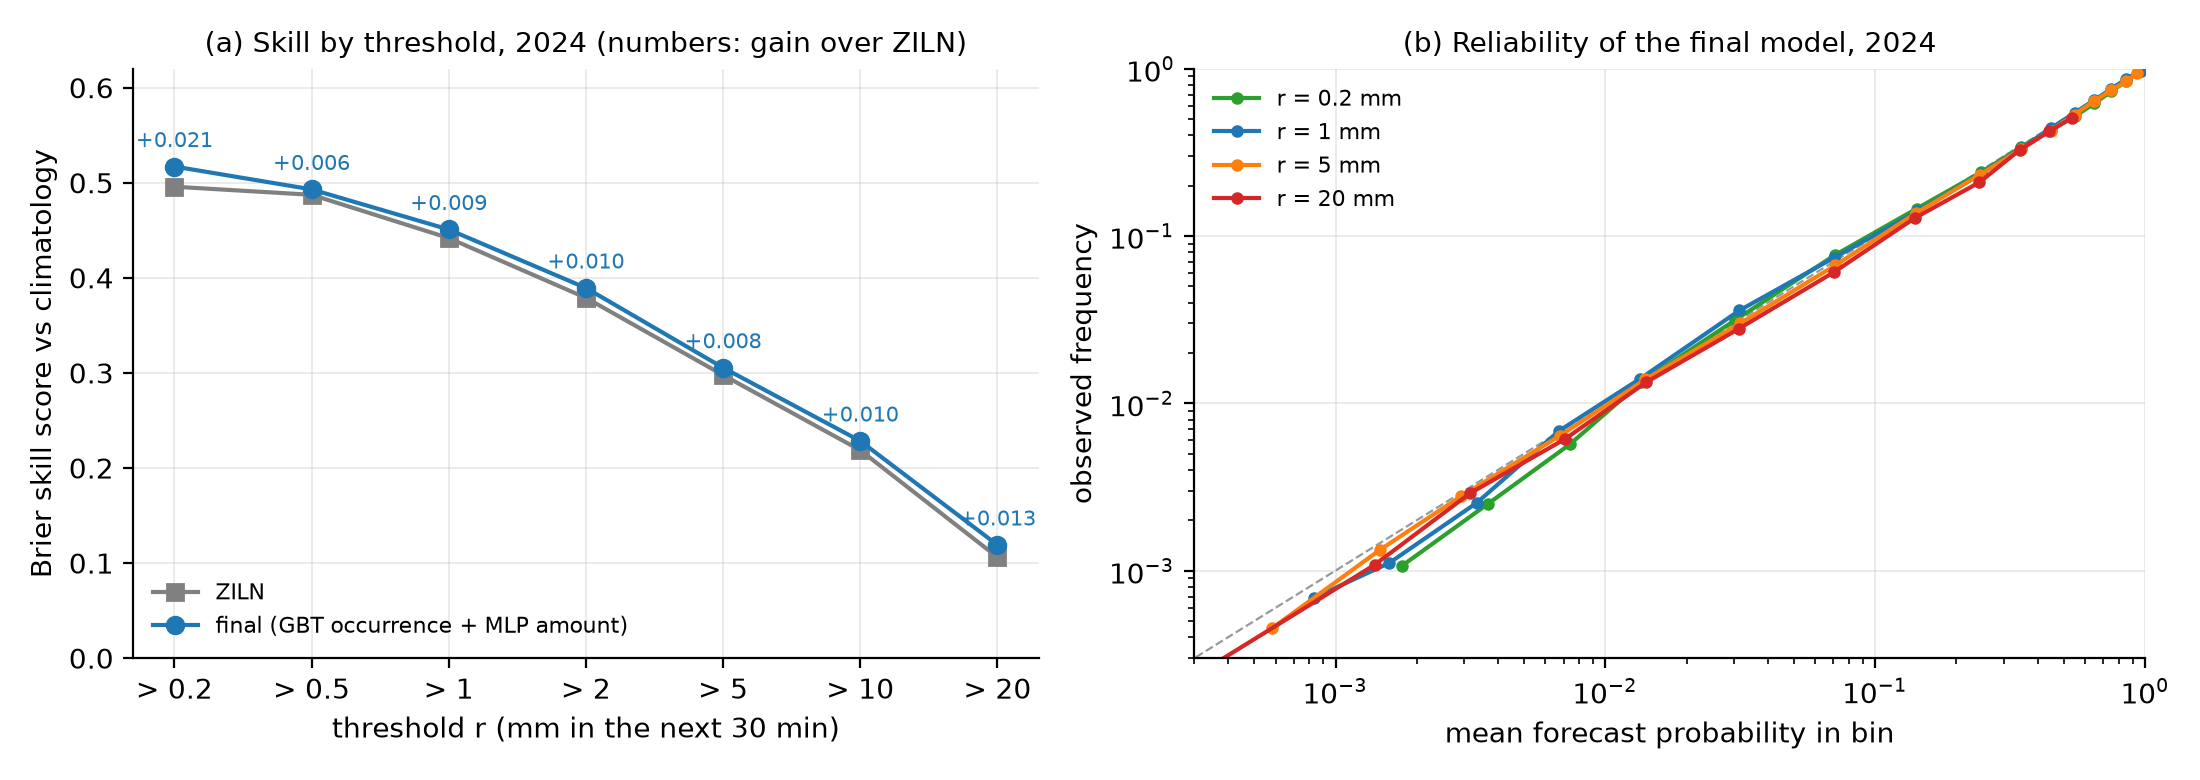
\includegraphics[width=\linewidth]{fig10_model_skill.png}
\caption{Final model on QC'd 2024. (a) Brier skill score by threshold, with the gain over ZILN. (b) Reliability: observed frequency against mean forecast in probability bins with at least 200 rows.}\label{fig:skill}
\end{figure}

\subsection{Where the model has skill}
Fig.~\ref{fig:cond} breaks the 1\mm{} skill down. It is similar across seasons (0.43--0.49) but varies with the hour. It is lowest at 12--14\,h (0.27--0.36), when afternoon storms begin, and at 01--02\,h, which have few events. The main division is the recent-rain state. When the station had rain in the last hour (9\% of rows, 74\% of events), the skill is 0.58. When the station and its eight neighbours were all dry (82\% of rows), it is 0.09: 12\% of events start from this state and cause 23\% of the Brier score, and the model can only raise their probability through the time of day and season. Here it over-predicts slightly (mean forecast 1.12 times the event rate). New convective cells that form overhead are the main limit on 30-minute skill with gauge data alone.

\begin{figure}[H]
\centering
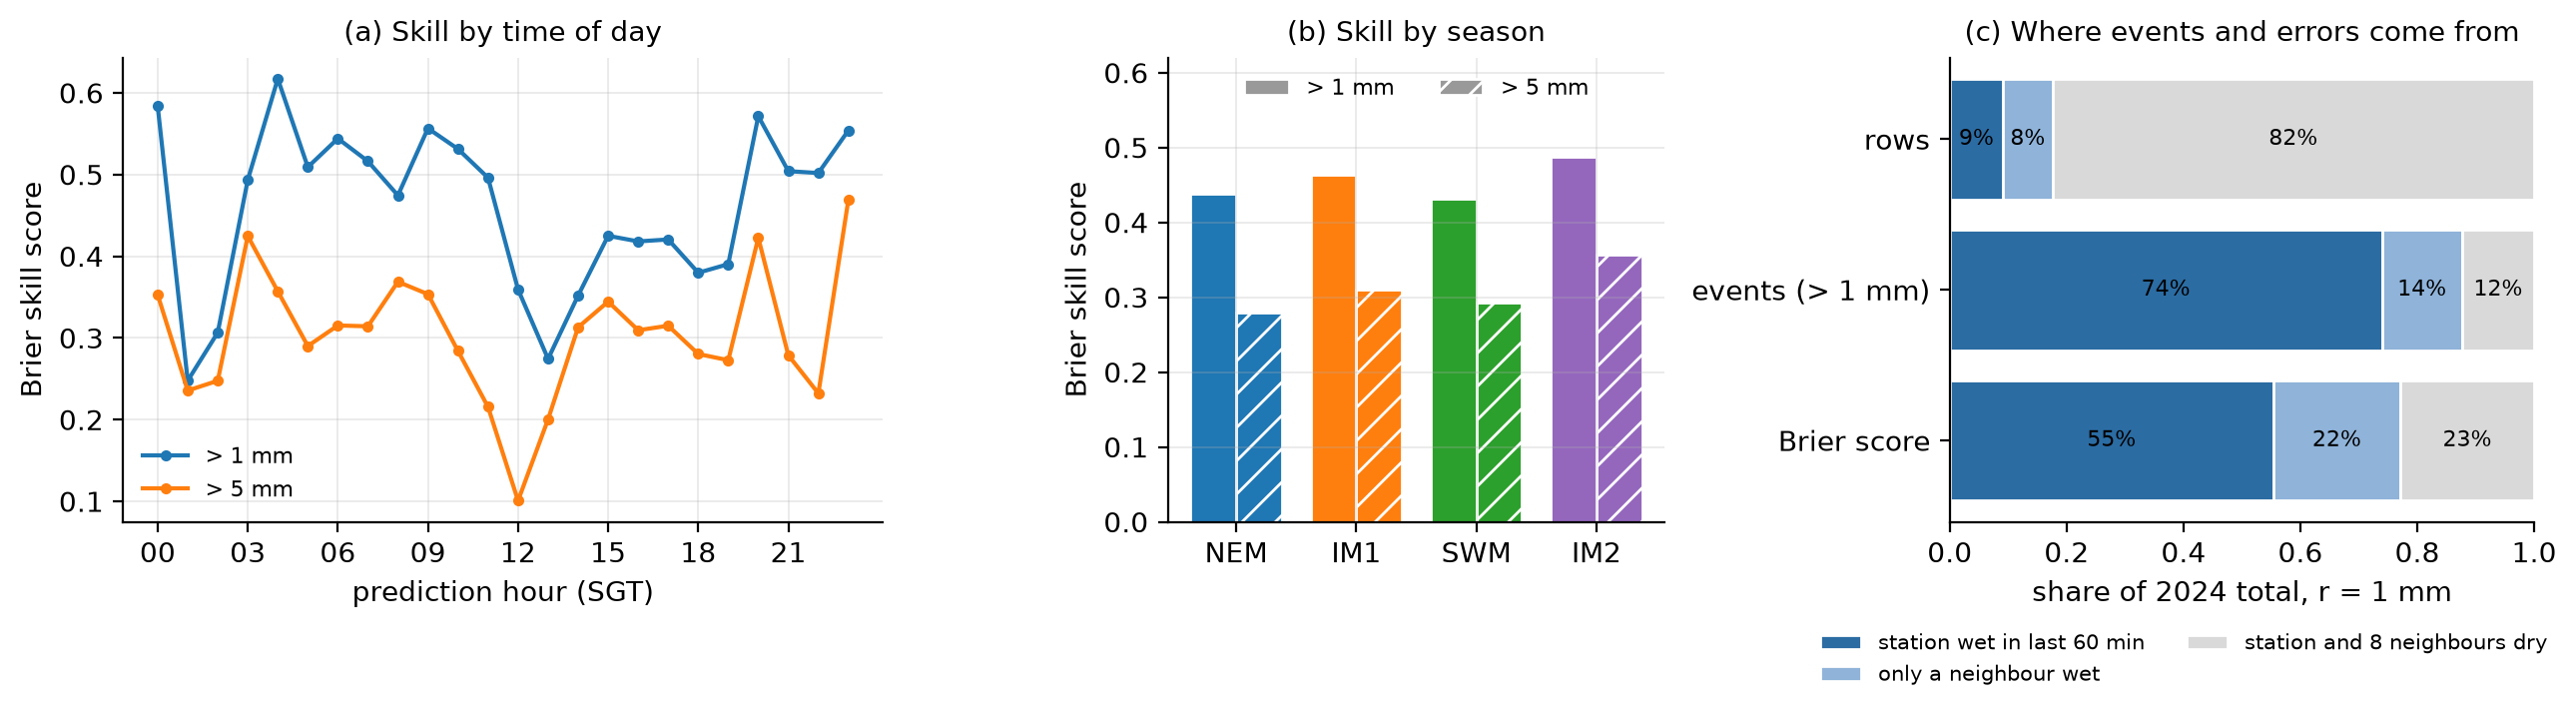
\includegraphics[width=\linewidth]{fig11_skill_by_condition.png}
\caption{Final model on QC'd 2024. (a, b) Brier skill score by prediction hour and season, all against the overall 2017--2022 climatology. (c) Shares of rows, events above 1\mm{} and Brier score by the rain in the last 60 minutes at the station and its eight nearest neighbours.}\label{fig:cond}
\end{figure}

\subsection{Robustness}
A second random seed changes no Brier skill score of the MLP by more than 0.0017, and every seed-to-seed bootstrap interval contains zero; the gains in Table~\ref{tab:final} are 3--12 times this spread. Refitting the MLP on the labels before the rounding fix changes the 2024 log score by less than $10^{-5}$. Training on QC'd data does not raise the scores: the ZILN model fitted to QC'd data scores 0.442 at 1\mm{} on the QC'd test rows, against 0.443 for the one fitted to the original data.

\section{Validity checks, limitations and insights}\label{sec:limits}
\subsection{Leakage and test-set use}
We checked the pipeline for information that would not be available at prediction time, and for choices that could flatter the test score:
\begin{itemize}[leftmargin=1.5em,itemsep=3pt]
\item \textbf{Features} use readings at or before the prediction time, and neighbour features lag by one slot. Features are built per year, so no training target reaches into 2023. All fitted transforms (station index, scaler, residual distributions) use the training years only. One look-ahead remains in metadata: the neighbour list of a year is built from all stations that report at some time that year, but a neighbour that has not yet started reporting is marked unavailable, never zero.
\item \textbf{Quality control} on the test year removes rows whose target window contains a flagged reading, which depends on the outcome. Scored on the original 2024 rows instead, the final model's Brier skill at 1\mm{} is 0.4505 against 0.4508 on the QC'd rows (Table~\ref{tab:compare}); at the other thresholds the difference is at most 0.0006, and for the ZILN model it is 0.0004. The QC rules were fixed before any model was trained on QC'd data and were not revised afterwards.
\item \textbf{Test-set use.} Every choice used 2023: features, hyperparameter set, error distribution, amount model and F1 cut-offs. However, 2024 is not a pristine holdout. Its scores were computed for every candidate during development, so the development process saw them. The 2023 scores give the same ranking (Table~\ref{tab:candidates}), and the differences between the leading models are small, so the reported 2024 scores should be read as estimates with roughly the bootstrap uncertainty.
\end{itemize}

\subsection{Limitations}
\begin{itemize}[leftmargin=1.5em,itemsep=3pt]
\item \textbf{Information, not the model, limits skill.} Every threshold-free candidate reaches ROC-AUC 0.94 at 1\mm, and the best amount model adds only 0.009 Brier skill. Storms that form overhead give no warning in gauge data; radar or satellite data would be needed.
\item \textbf{Eligible rows only.} Training and evaluation require a complete previous hour and target window. The model is not evaluated on stations with recent gaps, and a deployment would need a rule for them.
\item \textbf{QC is conservative.} The stuck-zero rule needs three wet neighbour days, so shorter stuck runs survive (39 runs of two days against about 6 expected by chance), and under-catch is not corrected (9 station-months collect less than 30\% of their neighbours' rain). Labels at multiples of 0.2\mm{} depend on gauge calibration of $\pm2\%$.
\item \textbf{One test year and eight years of climate.} 2024 was a near-average year. The Task~1 trends cannot be separated from year-to-year variability, and the station network changed in 2020.
\item \textbf{Local mode.} All jobs ran on one machine. The code uses only DataFrame and MLlib operations and should scale to a cluster, but we did not test one.
\end{itemize}

\subsection{Insights}
Rainfall in Singapore varies through how often it rains far more than how hard: frequency explains the dry year 2019 and the January maximum, while intensity peaks in the inter-monsoon thunderstorms. For prediction, this makes persistence and the recent state of nearby gauges the dominant information, and a model of the full rainfall distribution answers every threshold consistently and with calibrated probabilities.

\section{Reproduction and submitted files}
The README gives every command. Briefly, from \path{project2/}, with Java 17 and \texttt{pip install -r requirements.txt}:
\begin{lstlisting}[basicstyle=\footnotesize\ttfamily]
bash scripts/download_rainfall_data.sh && python scripts/verify_raw_data.py
bash scripts/run_pipeline.sh          # clean -> features -> neighbour features
python scripts/build_rich_features.py
bash scripts/run_qc_pipeline.sh       # QC -> data/interim_qc, data/processed_qc
python scripts/train_ziln.py --processed-dir data/processed_qc --feature-set rich \
    --occ-max-iter 120 --occ-step-size 0.2 --max-iter 100 --step-size 0.1 \
    --model-dir models/ziln_rich_qc
python scripts/train_amount_model.py --kind mlp --ziln-dir models/ziln_rich_qc \
    --processed-dir data/processed_qc --model-dir models/amount_mlp_qc
python scripts/evaluate_amount_models.py --ziln-dir models/ziln_rich_qc \
    --processed-dir data/processed_qc --amount-dirs models/amount_mlp_qc \
    --report reports/amount_models_qc_evaluation.json
python scripts/eda_patterns.py && python scripts/plot_eda.py      # Task 1
python scripts/diagnose_final_model.py && python scripts/plot_model.py   # Task 2 figures
\end{lstlisting}
The trained final model is in \path{models/ziln_rich_qc} (occurrence GBT, 3.5\,MB) and \path{models/amount_mlp_qc} (MLP, 0.2\,MB). Evaluation reports are in \path{reports/}, and figures in \path{reports/figures/}.

\section*{References and AI usage}
\begin{enumerate}[label={[\arabic*]},leftmargin=1.8em,itemsep=6pt]
\item\label{ref:1} National Environment Agency. \href{https://data.gov.sg/collections/2279/view}{Historical Rainfall across Singapore}, data.gov.sg, 2017--2024 annual datasets. Accessed October 2026.
\item\label{ref:2} Meteorological Service Singapore. \href{https://www.weather.gov.sg/climate-climate-of-singapore/}{Climate of Singapore}. Accessed October 2026.
\item\label{ref:3} Urban Redevelopment Authority. \href{https://data.gov.sg/datasets/d_4765db0e87b9c86336792efe8a1f7a66/view}{Master Plan 2019 Planning Area Boundary (No Sea)}, data.gov.sg. Accessed October 2026.
\item\label{ref:4} Apache Spark 4.0 documentation. \href{https://spark.apache.org/docs/4.0.1/ml-classification-regression.html}{MLlib: classification and regression}. Accessed October 2026.
\item\label{ref:5} X. Wang, T. Liu and J. Miao (2019). \href{https://arxiv.org/abs/1912.07753}{A deep probabilistic model for customer lifetime value prediction}. arXiv:1912.07753.
\item\label{ref:6} T. Gneiting and A. E. Raftery (2007). Strictly proper scoring rules, prediction, and estimation. \emph{Journal of the American Statistical Association} 102(477), 359--378.
\item\label{ref:7} H. R. Künsch (1989). The jackknife and the bootstrap for general stationary observations. \emph{Annals of Statistics} 17(3), 1217--1241.
\item\label{ref:8} J. Platt (1999). Probabilistic outputs for support vector machines and comparisons to regularized likelihood methods. In \emph{Advances in Large Margin Classifiers}, MIT Press.
\item\label{ref:9} Project source code. \href{https://github.com/Erchiusx/dsa5208/tree/master/project2}{Erchiusx/dsa5208, directory project2}. Report template: ElegantPaper 0.12 (LPPL 1.3c).
\item\label{ref:10} \textbf{AI usage.} \AIUsage
\end{enumerate}
\end{document}
